
\newcommand{\kZrememberedSampleLoops}{10}
\newcommand{\qZmaxLoops}{50}
\newcommand{\thetaZmaxCov}{0.1}
\newcommand{\readingClassFilesTime}{4755.32 \pm 141.66}
\newcommand{\queryCOVARIANTCOMPARETO}{$1$}
\newcommand{\speedupTCOVARIANTCOMPARETO}{4.4x}
\newcommand{\queryGCCALL}{$2$}
\newcommand{\speedupTGCCALL}{9.5x}
\newcommand{\queryPROTECTEDFIELD}{$3$}
\newcommand{\speedupTPROTECTEDFIELD}{9.8x}
\newcommand{\queryRUNFINALIZERSONEXIT}{$4$}
\newcommand{\speedupTRUNFINALIZERSONEXIT}{51x}
\newcommand{\queryNOTCLONEABLE}{$5$}
\newcommand{\speedupTNOTCLONEABLE}{61x}
\newcommand{\queryCOVARIANTEQUALS}{$6$}
\newcommand{\speedupTCOVARIANTEQUALS}{147x}
\newcommand{\queryFINALIZERNOTPROTECTED}{$7$}
\newcommand{\speedupTFINALIZERNOTPROTECTED}{1070x}
\newcommand{\queryDONTCATCHIMSE}{$8$}
\newcommand{\speedupTDONTCATCHIMSE}{12800x}
\newcommand{\queryURUNINITREADCALLEDFROMSUPERCONSTRUCTOR}{$9^R$}
\newcommand{\speedupTURUNINITREADCALLEDFROMSUPERCONSTRUCTOR}{0.9x}
\newcommand{\queryMSPKGPROTECT}{$10^R$}
\newcommand{\speedupTMSPKGPROTECT}{1.0x}
\newcommand{\querySICINNERSHOULDBESTATICANON}{$11^R$}
\newcommand{\speedupTSICINNERSHOULDBESTATICANON}{1.0x}
\newcommand{\queryITAINEFFICIENTTOARRAY}{$12^R$}
\newcommand{\speedupTITAINEFFICIENTTOARRAY}{1.1x}
\newcommand{\queryBXBOXINGIMMEDIATELYUNBOXEDTOPERFORMCOERCION}{$13^R$}
\newcommand{\speedupTBXBOXINGIMMEDIATELYUNBOXEDTOPERFORMCOERCION}{1.2x}
\newcommand{\queryDMILONGBITSTODOUBLEINVOKEDONINT}{$14^R$}
\newcommand{\speedupTDMILONGBITSTODOUBLEINVOKEDONINT}{1.3x}
\newcommand{\queryDPDOINSIDEDOPRIVILEGED}{$15^R$}
\newcommand{\speedupTDPDOINSIDEDOPRIVILEGED}{1.5x}
\newcommand{\queryMSSHOULDBEFINAL}{$16^R$}
\newcommand{\speedupTMSSHOULDBEFINAL}{1.8x}
\newcommand{\querySEBADFIELDINNERCLASS}{$17^R$}
\newcommand{\speedupTSEBADFIELDINNERCLASS}{6.9x}
\newcommand{\querySWSWINGMETHODSINVOKEDINSWINGTHREAD}{$18^R$}
\newcommand{\speedupTSWSWINGMETHODSINVOKEDINSWINGTHREAD}{13x}
\newcommand{\queryFIUSELESS}{$19^R$}
\newcommand{\speedupTFIUSELESS}{541x}
\newcommand{\MaxDevExp}{28.7}
\newcommand{\MaxStdErrExp}{9.1}
\newcommand{\minInvInterpOver}{0.3}
\newcommand{\geoMeanInterpOver}{1.2}
\newcommand{\maxInvInterpOver}{12.9}
\newcommand{\minInterpOver}{0.1}
\newcommand{\maxInterpOver}{3.4}
\newcommand{\minOptimTime}{3.5}
\newcommand{\avgOptimTime}{54.8}
\newcommand{\stdDevOptimTime}{85.5}
\newcommand{\maxOptimTime}{381.7}
\newcommand{\minOptimSpeedup}{1.2x}
\newcommand{\maxOptimSpeedup}{12800x}
\newcommand{\nSpeededUpQueries}{15}
\newcommand{\speedupBigThreshold}{5}
\newcommand{\nBigSpeededUpQueries}{10}
\newcommand{\randomQueryCount}{11}
\newcommand{\manualQueryCount}{8}
\newcommand{\queryCount}{19}
\newcommand{\avgSpeedupT}{12x}
\newcommand{\maxSpeedupT}{12800x}


\part{Optimizing Collection Queries by Reification}
\label{part:ch-aosd13}

\chapter{Introduction}
\label{sec:aosd13-intro}
\label{ch:aosd13-intro}
In-memory collections of data often need efficient processing. For on-disk
data, efficient processing is already provided by database management systems~(DBMS) thanks to
their query optimizers, which support many optimizations specific to the domain
of collections. Moving in-memory data to DBMSs, however,
typically does not improve performance~\citep{Stonebraker07}, and query optimizers cannot
be reused separately since DBMS are typically monolithic and their optimizers deeply integrated.
A few collection-specific optimizations, such as shortcut
fusion~\citep{Gill93shortcut}, are supported by compilers for purely
functional languages such as Haskell. However, the implementation techniques for
those optimizations do not
generalize to many other ones, such as support for indexes. In
general, collection-specific optimizations are not supported by the general-purpose
optimizers used by typical (JIT) compilers.

%Therefore, programs often manipulate collections using languages where automatic
%domain-specific optimizations are not supported, and thus perform some
%collection-related optimizations by hand.%~\citep{AOP}.

% High-level is missing. Maybe put that in the conclusion.
%Programmers would benefit from domain-specific
%optimizations which are not supported by
%current general-purpose optimizers.
%Such optimizations are supported instead by query optimizers in database
%management systems (DBMS). However, such query optimizers cannot be used on their own because
%database systems are usually monolithic; moving collection processing to a
%DBMS, instead, is not always appropriate nor easy since they are geared toward on-disk data and support a
%quite different data model: in-memory data is typically represented as an object
%graph, which is not easy to convert to flat relational data; specialized toolkit
%exist, but require a high amount of control from the programmer~\citep{Meijer11CoSQL}.
%%it is not trivial to convert in-memory data (object
%%graphs) to flat relational data, that is, to perform object-relational
%%mapping~\citep{Meijer11CoSQL}.
%A similar mismatch exists between SQL and most
%general-purpose programming languages: expressing general-purpose
%computations in SQL is therefore often problematic~\citep{Stonebraker07,Yu08}.
Therefore programmers, when needing
collection-related optimizations, perform them manually. To allow that, they are often forced to perform manual
inlining~\citep{Peyton-Jones02}.
But manual inlining
modifies source code by combining distinct functions together, while often distinct
functions should remain distinct, because they deal with different concerns, or
because one function need to be reused in a different context.
In either case, manual inlining reduces modularity --- defined here as the
ability to abstract behavior in a separate function (possibly part of a
different module) to enable reuse and improve understandability.%
%In general, to preserve modularity.
%When a function is separated because it is part of another module, manual
%inlining will reduce modularity.

%can reduce modularity.% and in particular violates \emph{information hiding}.
%Programs are partitioned in different modules, that is modularized, for many
%reasons, for instance to separate different implementation concerns and hide
%implementation details from one another. The smallest modularization
%Inlining combines together code from different functions
%Code fragments are divided in differen modules to hide implementation details between
%abstraction barriers.
%Manual inlining modifies source code by combining functions, even if it would
%be better to keep them distinct, because for instance they are part of different
%modules, or they have logically different goals.
%---we assume for some good reason, for instance because they are part of different modules.
%When two functions are logically distinct,

For these reasons, currently developers need to choose between modularity and
performance, as also highlighted by
\citet{AOP} on a similar example.
Instead, we envision that they should rely on an automatic optimizer performing inlining
and collection-specific optimizations. They would then achieve both performance and modularity.%
\footnote{In the terminology of \citet{AOP}, our goal is to be able to decompose
different \emph{generalized procedures} of a program according to its primary
decomposition, while separating the handling of some performance concerns. To
this end, we are modularizing these performance concerns into a
metaprogramming-based optimization module, which we believe
could be called, in that terminology, \emph{aspect}.}

One way to implement such an optimizer would be to extend the compiler of the language with a collection-specific optimizer, or
to add some kind of external preprocessor to the language. However, such solutions would be rather brittle (for instance, they lack
composability with other language extensions) and they would preclude optimization opportunities that arise only at runtime.

For this reason, our approach is implemented as an embedded domain-specific language (EDSL), that is, as a regular library.
We call this library \LoSDef. \LoS\ consists of a Scala EDSL for queries on collections based on the Scala collections API\@.
An expression in this EDSL produces at run time an \emph{expression tree} in the host language: a data structure which represents the query to execute, similar to an abstract syntax tree (AST) or a query plan. Thanks to the extensibility of Scala, expressions in this language look almost identical to expressions with the same meaning in Scala.
When executing the query, \LoS\ optimizes and compiles these expression trees for more efficient execution. Doing optimization at run time, instead of compile-time, avoids the need for control-flow analyses to determine which code will be actually executed~\citep{Chambers10}, as we will see later.

We have chosen Scala \citep{Odersky11book} to implement our library for two reasons: (i) Scala is a good meta-language for EDSLs, because it is syntactically
flexible and has a powerful type system, and (ii) Scala has a sophisticated collections library with an attractive syntax (for-comprehensions) to specify queries.

To evaluate \LoS, we study queries of the FindBugs tool~\citep{DBLP:journals/sigplan/HovemeyerP04}.
We rewrote a set of queries to use the Scala collections API and show that modularization incurs significant performance overhead. Subsequently, we consider versions of the same queries using \LoS{}.
We demonstrate that the automatic optimization can reconcile modularity and performance in many cases. Adding advanced optimizations such as indexing can even improve the performance of the analyses beyond the original non-modular analyses.

\section{Contributions and summary}
\label{sec:aosd13-contributions}
\label{sec:navigating-aosd13}

Overall, our main contributions in \cref{part:ch-aosd13} are the following:
\begin{itemize}
\item We illustrate the tradeoff between modularity and performance when manipulating collections, caused by the lack of domain-specific optimizations~(\cref{sec:motivation}). Conversely, we illustrate how domain-specific optimizations lead to more readable and more modular code (\cref{sec:solution}).
\item We present the design and implementation of \LoS, an embedded DSL for queries on collections in Scala (\cref{sec:implementation}).
%\LoS\ makes heavy usage of advanced Scala features to preserve the ``look and feel'' of native Scala queries
% and is hence a significant showcase for these features~(\cref{sec:implementation}).
 \item We evaluate \LoS\ to show that it supports writing queries that are at the same time modular and fast. We do so by re-implementing several code analyses of the FindBugs tool.
 The resulting code is more modular and/or more efficient, in some cases by orders of magnitude.
 In these case studies, we measured average speedups of \avgSpeedupT{} with a maximum of \maxSpeedupT{}~(\cref{sec:evaluation}).
\end{itemize}

\section{Motivation}
\label{sec:motivation}

In this section, we show how the absense of collection-specific optimizations
forces programmers to trade modularity against performance, which motivates our design of {\LoS} to resolve this conflict.

As our running example through the chapter, we consider representing and querying a simple in-memory bibliography. A book has, in our schema, a title, a publisher and a list of authors. Each author, in turn, has a first and last name. We represent authors and books as instances of the Scala classes \code{Author} and \code{Book} shown in Fig.~\ref{fig:schema}. The class declarations list the type of each field: Titles, publishers, and first and last names are all stored in fields of type \code{String}. The list of authors is stored in a field of type \code{Seq[Author]}, that is, a sequence of authors -- something that would be more complex to model in a relational database.
The code fragment also defines a collection of books named \code{books}.
\begin{figure}[htb]
\begin{lstlisting}
package schema
case class Author(firstName: String, lastName: String)
case class Book(title: String, publisher: String,
  authors: Seq[Author])

val books: Set[Book] = Set(
  new Book("Compilers: Principles, Techniques and Tools",
       "Pearson Education",
       Seq(new Author("Alfred V.", "Aho"),
           new Author("Monica S.", "Lam"),
           new Author("Ravi", "Sethi"),
           new Author("Jeffrey D.", "Ullman"))
  /* other books ... */)
\end{lstlisting}
\caption{Definition of the schema and of some content.}
\label{fig:schema}
\end{figure}

As a common idiom to query such collections, Scala provides \emph{for-comprehensions}.
For instance, the for\-/comprehension computing \code{records} in Fig.~\ref{fig:query} finds all books published by Pearson Education and yields, for each of those books, and for each of its authors, a record containing the book title, the full name of that author and the number of additional coauthors.
The \emph{generator} \code{book <- books} functions like a loop header: The remainder of the for-comprehension is executed once per book in the collection. Consequently, the \emph{generator} \code{author <- book.authors} starts a nested loop.
The return value of the for-comprehension is a collection of all yielded
records. Note that if a book has multiple authors, this for-comprehensions will
return multiple records relative to this book, one for each author.

\begin{figure}[htb]
\begin{lstlisting}
case class BookData(title: String, authorName: String,
  coauthors: Int)

val records =
  for {
    book <- books
    if book.publisher == "Pearson Education"
    author <- book.authors
  } yield new BookData(book.title,
                 author.firstName + " " +
                 author.lastName,
                 book.authors.size - 1)

def titleFilter(records: Set[BookData],
    keyword: String) =
  for {
    record <- records
    if record.title.contains(keyword)
  } yield (record.title, record.authorName)

val res = titleFilter(records, "Principles")
\end{lstlisting}
\caption{Our example query on the schema in Fig.~\ref{fig:schema}, and a function which postprocesses its result.}
\label{fig:query}
\end{figure}

We can further process this collection with another for-comprehension, possibly
in a different module. For example, still in Fig.~\ref{fig:query}, the function
\code{titleFilter} filters book titles containing the word "Principles", and
drops from each record the number of additional coauthors.

In Scala, the implementation of for-comprehensions is not fixed. Instead, the
compiler desugars a for-comprehension to a series of API calls, and different
collection classes can implement this API differently. Later, we will use this
flexibility to provide an optimizing implementation of for\-/comprehensions, but
in this section, we focus on the behavior of the standard Scala collections,
which implement for-comprehensions as loops that create intermediate
collections.

\subsection{Optimizing by Hand}

In the naive implementation in Fig.~\ref{fig:query} different concerns are separated, hence it is modular. However, it is also inefficient.
To execute this code, we first build the original collection and
only later we perform further processing to build the new result; creating the
intermediate collection at the interface between these functions is costly.
Moreover, the same book can appear in \code{records} more than once if the book has more than one author, but all of these duplicates have the same title. Nevertheless, we test each duplicate title separately whether it contains the searched \code{keyword}. If books have 4 authors on average, this means a slowdown of a factor of 4 for the filtering step.

In general, one can only resolve these inefficiencies by manually optimizing the query; however, we will observe that these manual optimizations produce less modular code.%
\footnote{%
The existing Scala collections API supports optimization, for instance through non-strict variants of the query operators (called `views' in Scala), but they can only
be used for a limited set of optimizations, as we discuss in \cref{sec:relwork}.}

To address the first problem above, that is, to avoid creating intermediate collections, we can manually inline \code{titleFilter} and \code{records}; we obtain two nested for\-/comprehensions.
Furthermore, we can \emph{unnest} the inner one~\citep{Fegaras00}.

To address the second problem above, that is, to avoid testing the same title multiple times, we \emph{hoist} the filtering step, that is, we change the order of the processing steps in the query to first look for \code{keyword} within \code{book.title} and then iterate over the set of authors. This does not change the overall semantics of the query because the filter only accesses the title but does not depend on the author. In the end, we obtain the code in Fig.~\ref{fig:titleFilterho2}. The resulting query processes the title of each book only once. Since filtering in Scala is done lazily, the resulting query avoids building an intermediate collection.

This second optimization is only possible after inlining and thereby reducing the modularity of the code, because it mixes together processing steps from \code{titleFilter} and from the definition of \code{records}. Therefore, reusing the code creating records would now be harder.

To make \code{titleFilterHandOpt} more reusable, we could turn the publisher name into a parameter.
However, the new versions of \code{titleFilter} cannot be reused as-is if some details of the inlined code change; for instance, we might need to filter publishers differently or not at all. On the other hand, if we express queries modularly, we might lose some opportunities for optimization. The design of the collections API, both in Scala and in typical languages, forces us to manually optimize our code by repeated inlining and subsequent application of query optimization rules, which leads to a loss of modularity.

\begin{figure}[htb]
\begin{lstlisting}
def titleFilterHandOpt(books: Set[Book],
                        publisher: String,
                        keyword: String) =
  for {
    book <- books
    if book.publisher == publisher && book.title.contains(keyword)
    author <- book.authors
  } yield (book.title, author.firstName + " " + author.lastName)
val res = titleFilterHandOpt(books,
  "Pearson Education", "Principles")
\end{lstlisting}
\caption{Composition of queries in Fig.~\ref{fig:query}, after inlining, query unnesting and hoisting.}
\label{fig:titleFilterho2}
\end{figure}


% XXX HACK
%\section{Automatic optimization with \textsc{\textbf{SQuOpt}}}
% Does not work well
\chapter{Automatic optimization with SQuOpt}

\label{ch:aosd13-solution}
\label{sec:solution}
The goal of {\LoS} is to let programmers write queries modularly and at a high level of abstraction and deal with optimization by a dedicated domain-specific optimizer. In our concrete example,
programmers should be able to write queries similar to the one in Fig.~\ref{fig:query}, but get the efficiency of the one in Fig.~\ref{fig:titleFilterho2}.
To allow this, {\LoS} overloads for-comprehensions and other constructs, such as string concatenation with \code{+} and field access \code{book.author}. Our overloads of these constructs reify the query as an expression tree. {\LoS} can then optimize this expression tree and execute the resulting optimized query.
Programmers explicitly trigger processing by {\LoS}, by adapting their queries as we describe in next subsection.

\section{Adapting a Query}
\label{subsec:adaptingaquery}
\begin{figure}
\centering
\begin{lstlisting}
import squopt._
import schema.squopt._

val recordsQuery =
  for {
    book <- books.asSquopt
    if book.publisher ==# "Pearson Education"
    author <- book.authors
  } yield new BookData(book.title,
    author.firstName + " " + author.lastName,
    book.authors.size - 1)

// ...
val records = recordsQuery.eval

def titleFilterQuery(records: Exp[Set[BookData]], keyword: Exp[String]) =
  for {
    record <- records
    if record.title.contains(keyword)
  } yield (record.title, record.authorName)

val resQuery = titleFilterQuery(recordsQuery, "Principles")
val res = resQuery.optimize.eval
\end{lstlisting}
\caption{\LoS\ version of Fig.~\ref{fig:query}; \code{recordsQuery} contains a reification of the query, \code{records} its result.}
\label{fig:reifiedQuery}
\end{figure}

To use {\LoS} instead of native Scala queries, we first assume that the query
does not use side effects and is thus \emph{purely functional}. We argue that purely functional queries are more
declarative. Side effects are used to improve performance, but
\LoS\ makes that unnecessary through automatic optimizations. In fact, the lack
of side effects enables more optimizations.

% KO: commented this out, let's not be too technical here
%There is one exception: logical operators
%(\code{&&} and \code{||}) are guaranteed to be short-circuiting in \LoS{},
%unlike in purely functional code; thus, code like \code{foo != null && foo.bar}
%remains valid.
% PG: also, that's not even strictly true.

%To simplify optimizations, the optimizer assumes no side effects are performed, and
In Fig.~\ref{fig:reifiedQuery} we show a version of our running example adapted to use {\LoS}. We first discuss changes to \code{records}.
To enable {\LoS}, a programmer needs to (a) import the \LoS\
library, (b) import some wrapper code specific to the types the collection
operates on, in this case \code{Book} and \code{Author} (more about that later), (c) convert explicitly the native Scala collections involved to collections of our framework by a call to \code{asSquopt}, (d) rename a few operators such as \code{==} to \code{==#} (this is necessary due to some Scala limitations), and (e) add a separate step where the query is evaluated (possibly after optimization). All these changes are lightweight and mostly of a  syntactic nature.

%Expressing a query through {\LoS} allows the query to benefit from various optimizations. Even if the query definition is split into different modules, optimizations work on the complete query definition, and thus cross modularity boundaries: the optimizer considers information defined in different modules to determine how to best optimize the query.
% Conclusion of the section.
%In general, a program in a deeply embedded DSL can benefit from the advantages of metaprogramming
% Idea 1: a DS-O can significantly improve performance, but also perform non-modular optimizations

%To trigger this optimization, we also express the second part of the running example with {\LoS} and explicitly call \lstinline!optimize! before running the query.

For parameterized queries like \code{titleFilter}, we need to also adapt type annotations.
The ones in \code{titleFilterQuery} reveal some details of our implementation:
Expressions that are reified have type \code{Exp[T]} instead of \code{T}.
As the code shows, \code{resQuery} is optimized before compilation. This call will perform the optimizations that we previously did by hand
and will return a query equivalent to that in Fig.~\ref{fig:titleFilterho2}, after verifying their safety conditions. For instance,
after inlining, the filter \code{if book.title.contains(keyword)} does not reference \code{author}; hence, it is safe to hoist.
Note that checking this safety condition would not be possible without reifying the predicate. For instance, it would
not be sufficient to only reify the calls to the collection API, because the predicate is represented as a boolean function parameter.
In general, our automatic optimizer inspects the whole reification of the query implementation to check that optimizations
do not introduce changes in the overall result of the query and are therefore safe.

\section{Indexing}
%We reuse path indexes~\citep{Bertino89}.
%\pg{We have no example which shows a hierarchical index, nor do we say we use
%path indexes, nor do we cite the paper (citation key Bertino89). Is that OK?}
% PG: yes at least for now, because of space reasons.

{\LoS} also supports the transparent usage of indexes. Indexes can further improve the efficiency of queries, sometimes by orders of magnitude.
In our running example, the query scans all books to look for the ones having the right publisher. To speed up this query, we can preprocess \code{books} to build an index, that is, a dictionary mapping, from each publisher to a collection of all the books it published. This index can then be used to answer the original query without scanning all books.

We construct a \emph{query} representing the desired dictionary, and inform the optimizer that it should use this index where appropriate:
\begin{lstlisting}
val idxByPublisher = books.asSquopt.indexBy(_.publisher)
Optimization.addIndex(idxByPublisher)
\end{lstlisting}

The \code{indexBy} collection method accepts a function that maps a collection element to a key; \code{coll.indexBy(key)} returns a dictionary mapping each key to the collection of all elements of \code{coll} having that key. Missing keys are mapped to an empty collection.%
\footnote{For readers familiar with the Scala collection API, we remark that the only difference with the standard \code{groupBy} method is the handling of missing keys.}
\code{Optimization.addIndex} simply preevaluates the index and updates a dictionary mapping the index to its preevaluated result.

% PG: this explanation is too simplified, explain this better later.
%In {\LoS}, the user is responsible for creating indexes, in form of \emph{queries} representing the desired dictionaries,
%and registering them.
%The automatic optimizer is responsible for using registered indexes where possible to speed up queries.
%In \LoS, an index is defined as a query which returns a map%
%% from the index key to the rest of the collection,
%, usually by calling the \code{indexBy} operator.
%This query is added to a collection of available
%indexes that are available for optimizing queries.

A call to \code{optimize} on a query will then take this index into account and rewrite the query to perform index lookup instead of scanning, if possible. For instance, the code in Fig.~\ref{fig:reifiedQuery} would be transparently rewritten by the optimizer to a query similar to the following:
\begin{lstlisting}
val indexedQuery =
  for {
    book <- idxByPublisher("Pearson Education")
    author <- book.authors
  } yield new BookData(book.title,
    author.firstName + " " + author.lastName,
    book.authors.size - 1)
\end{lstlisting}
Since dictionaries in Scala are functions, in the above code, dictionary lookup on \code{idxByPublisher} is represented simply as function application. The above code iterates over books having the desired publisher, instead of scanning the whole library, and performs the remaining computation from the original query. Although the index use in the listing above is notated as
\code{idxByPublisher("Pearson Education")}, only the cached result of evaluating the index is used when
the query is executed, not the reified index definition.

This optimization could also be performed manually, of course, but the queries are on a higher abstraction level and more maintainable if indexing is defined separately and applied automatically.
Manual application of indexing is a crosscutting concern because adding or removing an index affects potentially many queries.
\LoS\ does not free the developer from the task of assessing which index will `pay off' (we have not considered
automatic index creation yet), but at least it becomes simple to add or remove an index, since the application
of the indexes is modularized in the optimizer.

%For instance, the same index can be useful in many different queries; applying it manually in all queries leads to undesirable redundancy which is hard to maintain.

%Did we improve performance? Scanning a table of $n$ elements takes $\Theta(n)$, while a dictionary lookup takes $\Theta(1)$ or $\Theta(\log n)$ depending on the dictionary implementation; hence, we changed the complexity class of the query. On the other hand, we need to build the index in the first place, with a cost of at least $\Omega(n)$ (when representing the index as a hash map) and at most $O(n \log n)$ (when representing the index as a balanced tree); building such an index is convenient only if we use it often enough, for instance for many similar lookups. Thus, we cannot decide whether to use an index in a query based only on the query itself; similarly to databases, we need to consider all queries together to decide that. The decision to add an index is therefore non-modular; to limit its impact, it should be possible to implement it by doing a local change (creating and registering the index), rather than by altering all queries which should use that index.


%\pg{Exemplify join optimization? Better just cite~\citep{Willis06JQL} about it; they don't report great results IIRC, unlike their next version,~\citep{Willis08}.}

\chapter{Implementing SQuOpt}
\label{ch:aosd13-implementation}
\label{sec:implementation}

After describing how to use {\LoS}, we explain how \LoS{} represents queries internally and optimizes them.
\begin{techrep}
Here we give only a brief overview of our implementation technique; it is described in more detail
in \cref{sec:intfScala}.
\end{techrep}
\begin{nontechrep}
We give only a brief overview of our implementation technique; it is described in more detail
in a technical report that accompanies this paper~\citep{GiarrussoEtAl2012ReifyTR}.
\end{nontechrep}

\section{Expression Trees}
\label{sec:representation}
In order to analyze and optimize collection queries at runtime, {\LoS} reifies their syntactic structure as \emph{expression trees}.
The expression tree reflects the syntax of the query after desugaring, that is, after for-comprehensions have been replaced by API calls.
For instance, \code{recordsQuery} from Fig.~\ref{fig:reifiedQuery} points to the
following expression tree (with some boilerplate omitted for clarity):

\begin{lstlisting}
new FlatMap(
  new Filter(
    new Const(books),
    v2 => new Eq(new Book_publisher(v2),
                new Const("Pearson Education"))),
    v3 => new MapNode(
          new Book_authors(v3),
          v4 => new BookData(
                 new Book_title(v3),
                 new StringConcat(
                   new StringConcat(
                     new Author_firstName(v4),
                     new Const(" ")),
                   new Author_lastName(v4)),
                 new Plus(new Size(new Book_authors(v3)),
                          new Negate(new Const(1))))))
\end{lstlisting}

The structure of the for-comprehension is encoded with the \code{FlatMap}, \code{Filter} and \code{MapNode} instances. These classes correspond to the API methods that for-comprehensions get desugared to. {\LoS} arranges for the implementation of \code{flatMap} to construct a \code{FlatMap} instance, etc.
The instances of the other classes encode the rest of the structure of the collection query, that is, which methods are called on which arguments. On the one hand, {\LoS} defines classes such as \code{Const} or \code{Eq} that are generic and applicable to all queries. On the other hand, classes such as \code{Book_publisher} cannot be predefined, because they are specific to the user-defined types used in a query. {\LoS} provides a small code generator, which creates a case class for
each method and field of a user-defined type. Functions in the query are represented by functions that
create expression trees; representing functions in this way is frequently called higher-order
abstract syntax \citep{Pfenning88hoas}.

We can see that the reification of this code corresponds closely to an abstract
syntax tree for the code which is executed; however, many calls to specific
methods, like \code{map}, are represented by special nodes, like \code{MapNode}, rather
than as method calls.
For the optimizer it becomes easier to match and transform those
nodes than with a generic abstract syntax tree.

Nodes for collection operations are carefully defined by hand to provide them
highly generic type signatures and make them reusable for all collection types.
In Scala, collection operations are highly polymorphic; for instance, \code{map}
has a single implementation working on all collection types, like \code{List},
\code{Set}, and we similarly want to represent all usages of \code{map} through
instances of a single node type, namely \code{MapNode}. Having separate nodes \code{ListMapNode}, \code{SetMapNode} and so
on would be inconvenient, for instance when writing the optimizer.
However, \code{map}
on a \code{List[Int]} will produce another \code{List}, while on a \code{Set} it
will produce another \code{Set}, and so on for each specific collection type (in
first approximation); moreover, this is guaranteed statically by the type of
\code{map}. Yet, thanks to advanced typesystem features, \code{map} is defined
only once avoiding redundancy, but has a type polymorphic enough to guarantee
statically that the correct return value is produced.
Since our tree representation is strongly typed, we need to have a similar level
of polymorphism in \code{MapNode}. We achieved this by extending the techniques
described by \citet{odersky2009fighting}, as detailed in our technical report%
~\citep{GiarrussoEtAl2012ReifyTR}.

We get these expression trees by using Scala implicit conversions in a particular style, which we adopted from
\citet{rompf2010lightweight}. Implicit conversions allow to add, for each method
\code{A.foo(B)}, an overload of \code{Exp[A].foo(Exp[B])}. Where a value of
type \code{Exp[T]} is expected, a value of type \code{T} can be used thanks to
other implicit conversions, which wrap it in a \code{Const} node. The initial call of \code{asSquopt} triggers the application of the implicit conversions by
converting the collection to the leaf of an expression tree.

It is also possible to call methods that do not return expression trees; however, such method calls would
then only be represented by an opaque \code{MethodCall} node in the expression tree, which means that the code
of the method cannot be considered in optimizations.

Crucially, these expression trees are generated at runtime. For instance,
the first \code{Const} contains a reference to the actual collection of books to which \code{books} refers.
If a query uses another query, such as \code{records} in Fig.~\ref{fig:reifiedQuery}, then
the subquery is effectively \emph{inlined}. The same holds for method calls inside queries: If these methods
return an expression tree (such as the \code{titleFilterQuery} method in Fig.~\ref{fig:reifiedQuery}), then
these expression trees are inlined into the composite query. Since the reification happens at runtime, it is not
necessary to predict the targets of dynamically bound method calls: A new (and possibly different) expression tree
is created each time a block of code containing queries is executed.

Hence, we can say that expression trees represent the computation which is going to be executed
after inlining; control flow or virtual calls in the original code typically
disappear---especially if they manipulate the query as a whole.
This is typical of deeply embedded DSLs like ours, where code instead of performing
computations produces a representation of the computation to
perform~\citep{elliott03compiling, Chambers10}.

This inlining can duplicate computations; for instance, in this
code:
\begin{lstlisting}
val num: Exp[Int] = 10
val square = num * num
val sum = square + square
\end{lstlisting}
evaluating \code{sum} will evaluate \code{square} twice.
\citet{elliott03compiling} and we avoid this using common-subexpression
elimination.

\section{Optimizations}

Our optimizer currently supports several algebraic optimizations.
Any query and in fact every reified expression can be optimized by calling the \code{optimize} function on it. The ability to optimize reified expressions that are not queries is
useful; for instance, optimizing a function that produces a query is similar to a ``prepared statement''
in relational databases.

The optimizations we implemented are mostly standard in compilers~\citep{DBLP:books/mk/Muchnick1997} or databases:

\begin{itemize}
\item \emph{Query unnesting} merges a nested query into the containing
one~\citep{Fegaras00,Grust99How}, replacing for instance
\begin{lstlisting}
for {val1 <- (for {val2 <- coll} yield f(val2))}
  yield g(val1)
\end{lstlisting}
with
\begin{lstlisting}
for {val2 <- coll; val1 = f(val2)} yield g(val1)
\end{lstlisting}
%A more complex example was in \ref{fig:titleFilterho2}.
\item \emph{Bulk operation fusion} fuses higher-order operators on collections.
% How to explain it?
%This allows optimizations across the arguments of different operators.
\item \emph{Filter hoisting} tries to apply filters as early as possible; in
database query optimization, it is known as selection pushdown. For filter hoisting, it
is important that the full query is reified, because otherwise the dependencies of the filter condition
cannot be determined.
\item
%To reduce data abstraction overhead, we
We reduce during optimization
tuple/case class accesses: For instance,
\code{(a, b)._1} is simplified to \code{a}. This is important because
the produced expression does not depend on \code{b}; removing this false
dependency can allow, for instance, a filter containing this expression to be
hoisted to a context where \code{b} is not bound.
%In turn, this allows a filter of form \code{b => (a, b)._1} to
\item \emph{Indexing} tries to apply one or more of the available indexes to speed up the query.
\item \emph{Common subexpression elimination (CSE)} avoids that the same computation
is performed multiple times; we use techniques similar to
\citet{rompf2010lightweight}.
\item Smaller optimizations include constant folding, reassociation of
associative operators and
      %beta-reduction,  Klaus: this may raise too many questions
      removal of identity maps (\code{coll.map(x => x)}, typically generated by
      the translation of for-comprehensions).
\end{itemize}
%The optimizations are applied iteratively until no more optimizations are applicable.
Each optimization is applied recursively bottom-up until it does not trigger
anymore; different optimizations are composed in a fixed pipeline.

Optimizations are only guaranteed to be semantics\-/preserving if queries obey the
restrictions we mentioned: for instance, queries should not involve
side-effects such as assignments or I/O, and all collections used in queries
should implement the specifications stated in the collections API\@. Obviously the choice of optimizations involves many tradeoffs; for that reason
we believe that it is all the more important that the optimizer is not
hard-wired into the compiler but implemented as a library, with potentially
many different implementations.

To make changes to the optimizer more practical, we designed our query
representation so that optimizations are easy to express; restricting to pure
queries also helps. For instance, filter fusion can be implemented in few lines of code:
just match against expressions of form \code{coll.filter(pred2).filter(pred1)}
and rewrite them:%
\footnote{\code{Sym} nodes are part of the boilerplate we omitted earlier.}
\begin{lstlisting}
  val mergeFilters = ExpTransformer {
    case Sym(Filter(Sym(Filter(collection, pred2)), pred1)) =>
      coll.filter(x => pred2(x) && pred1(x))
  }
\end{lstlisting}
A more complex
optimization such as filter hoisting requires only 20 lines of code.

We have implemented a prototype of the optimizer with the mentioned
optimizations. Many additional algebraic optimizations can be added in future
work by us or others; a candidate would be loop hoisting, which moves out of
loops arbitrary computations not depending on the loop variable (and not just filters).
With some changes to the optimizer's architecture, it would also be possible to perform cost-based and dynamic optimizations.

\section{Query Execution}
\label{sec:execution}
Calling the \code{eval} method on a query will convert it to executable
bytecode; this bytecode will be loaded and invoked by using Java reflection.
We produce a thunk that, when evaluated, will execute the
generated code.

In our prototype we produce bytecode by converting expression trees to
Scala code and invoking on the result the Scala compiler, \texttt{scalac}. Invoking
\texttt{scalac} is typically quite slow, and we currently use caching to limit
this concern; however, we believe it is merely an engineering problem to
produce bytecode directly from expression trees, just as compilers do.

Our expression trees contain native Scala values wrapped in \code{Const} nodes,
and in many cases one cannot produce Scala program text evaluating to the same value.
To allow executing such expression trees we need to implement cross-stage
persistence (CSP): the generated code will be a function, accepting the actual
values as arguments~\citep{rompf2010lightweight}. This allows sharing the compiled
code for expressions which differ only in the embedded values.

More in detail, our compilation algorithm is as follows.
(a) We implement CSP by replacing embedded Scala values by references to the
function arguments; so for instance \code{List(1, 2, 3).map(x => x + 1)} becomes
the function \code{(s1: List[Int], s2: Int) => s1.map(x => x + s2)}.
(b) We look up the produced expression tree, together with the types of the
constants we just removed, in a cache mapping to the generated classes. If the
lookup fails we update the cache with the result of the next steps.
(c) We apply CSE on the expression.
(d) We convert the tree to code, compile it and load the generated code.

\smartParagraph{Preventing errors in generated code}
Compiler errors in generated code are typically a concern; with \LoS{}, however,
they can only arise due to implementation bugs in \LoS{} (for instance in
pretty-printing, which cannot be checked statically), so they do not concern
users.
Since our query language and tree representation are statically typed,
type-incorrect queries will be rejected statically.
For instance, consider again \code{idxByPublisher}, described previously:
\begin{lstlisting}
val idxByPublisher = books.asSquopt.indexBy(_.publisher)
\end{lstlisting}
Since \code{Book.publisher} returns a \code{String}, \code{idxByPublisher} has
type \code{Exp[Map[String, Book]]}. Looking up a key of the wrong type, for
instance by writing \code{idxByPublisher(book)} where \code{book: Book}, will
make \texttt{scalac} emit a static type error.

\chapter{A deep EDSL for collection queries}
\label{ch:aosd13-caseStudy}
\label{sec:caseStudy}
In this chapter we discuss collections as a \emph{critical} case
study~\citep{flyvbjerg06five} for deep DSL embedding.

As discussed in the previous chapter, to support optimizations we require a deep embedding of the collections DSL\@.

While the basic idea of deep embedding is well known, it is not obvious how to realize deep embedding
when considering the following additional goals:

\begin{itemize}
\item To support users adopting \LoS, a generic \LoS\ query should share the ``look and feel'' of the ordinary collections API: In particular, query syntax should remain mostly unchanged. In our case, we want to preserve  Scala's \emph{for-comprehension}\footnote{Also known as \emph{for expressions}~\citep[Ch.~23]{Odersky11book}.} syntax and its notation
 for anonymous functions.
 %IDE services for native Scala queries (such as syntax highlighting or
 %reference resolving) should also work with \LoS\ queries.
 % Paolo: That seems irrelevant, this is guaranteed by all deep embeddings.
 \item Again to support users adopting \LoS, a generic \LoS\ query should not only share the syntax of the ordinary collections API; it should also be well-typed if and only if the corresponding ordinary query is well-typed.
 This is particularly challenging in the Scala collections
 library due to its deep integration with advanced type-system features, such as higher-kinded generics
 and implicit objects~\citep{odersky2009fighting}. For instance, calling \code{map} on a \code{List} will return a \code{List}, and calling \code{map} on a \code{Set}
 will return a \code{Set}. Hence the object-language representation and the
 transformations thereof should be as ``typed'' as possible. This precludes, among others, a first-order
 representation of object-language variables as strings.
 \item \LoS\ should be interoperable with ordinary Scala code and Scala collections. For instance, it should
 be possible to call normal non-reified functions within a \LoS\ query, or mix native Scala queries and \LoS\ queries.
%KO: commented this out because we now have the RW section early
%\item \LINQ\ also reifies queries by relying on built-in support for deep embedding (in the form of expression trees); we want instead to express deep embedding as a library using general-purpose language constructs of more general applicability.
 \item The performance of \LoS\ queries should be reasonable even without optimizations. A non-optimized \LoS\ query
 should not be dramatically slower than a native Scala query. Furthermore, it should be possible to create new queries at run time and execute them without excessive overhead.
 This goal limits the options of applicable interpretation or compilation techniques.
\end{itemize}
\chk{these goals are not really justified, but that may be too late to change}
 
We think that these challenges characterize deep embedding of queries on collections as a \emph{critical} case study~\citep{flyvbjerg06five} for DSL embedding.
That is, it is so challenging that embedding techniques successfully used in this case are likely to be successful on a broad range of other DSLs.
From the case study, we report the successes and failures of achieving these goals in \LoS. 


\section{Implementation: Expressing the interface in Scala}
\label{ch:aosd13-intfScala}
\label{sec:intfScala}
%\section{The DSEL interface: embedding Scala expressions}
% Scala-virtualized has no polymorphic lift, unlike us.
% 2. Embedding collections into Scala
% When does one need asSquopt?
To optimize a query as described in the previous section, {\LoS} needs to reify, optimize and execute queries. 
Our implementation assigns responsibility for these steps to three main components: A generic library for reification and execution of general Scala expressions, a more specialized library for reification and execution of query operators, and a dedicated query optimizer.
Queries need then to be executed through either compilation (already discussed in
Sec.~\ref{sec:execution}) or interpretation (to discuss in Sec.~\ref{sec:interpretation}).
We describe the implementation in more detail in the rest of this section. The full implementation is also available online\footnote{\url{http://www.informatik.uni-marburg.de/~pgiarrusso/SQuOpt}}.
%\url{https://github.com/Blaisorblade/SQuOpt}.

A core idea of {\LoS} is to reify Scala code as a data structure in memory. A programmer could directly create instances of that data structure, but we also provide a more convenient interface based on advanced Scala features such as implicit conversions and type inference. That interface allows to automatically reify code with a minimum of programmer annotations, as shown in the examples in Sec.~\ref{sec:solution}. Since this is a case study on Scala's support for deep embedding of DSLs, we also describe in this section how Scala supports our task. In particular, we report on techniques we used and issues we faced.

%\pg{Somewhere: Contrast a bit with LMS - we are more open, provide less compile-time safety, etc.; motivate differences. This section risks being boring, explain why it is not.}
\section{Representing expression trees}
\label{subsec:repexptrees}
In the previous section, we have seen that expressions that would have type \code{T} in a native Scala query are reified and have type \code{Exp[T]} in \LoS. The generic type \code{Exp[T]} is the base for our reification of Scala expression as expression trees, that is, as data structures in memory. We provide a subclass of \code{Exp[T]} for every different form of expression we want to reify. For example, in Fig.~\ref{fig:query} the expression \code{author.firstName + " " + author.lastName} must be reified even though it is not collection-related, for otherwise the optimizer could not see whether \code{author} is used. Knowing this is needed for instance to remove variables which are bound but not used. Hence, this expression is reified as \code{StringConcat(StringConcat(AuthorFirstName(author), Const(" ")), AuthorLastName(author))}. This example uses the constructors of the following subclasses of \code{Exp[T]} to create the expression tree.

\begin{lstlisting}
case class Const[T](t: T) extends Exp[T]

case class StringConcat(str1: Exp[String],
                        str2: Exp[String])
  extends Exp[String]

case class AuthorFirstName(t: Exp[Author])
  extends Exp[String]

case class AuthorLastName(t: Exp[Author])
  extends Exp[String]
\end{lstlisting}

Expression nodes additionally implement support code for tree traversals to support optimizations, which we omit here.

This representation of expression trees is well-suited for a representation of the structure of expressions in memory and also for pattern matching (which is automatically supported for case classes in Scala), but inconvenient for query writers. In fact, in Fig.~\ref{fig:reifiedQuery}, we have seen that {\LoS} provides a much more convenient front-end: The programmer writes almost the usual code for type \code{T} and {\LoS} converts it automatically to \code{Exp[T]}.

\section{Lifting first-order expressions}

We call the process of converting from \code{T} to \code{Exp[T]} \emph{lifting}. Here we describe how we lift first-order expressions -- Scala expressions that do
not contain anonymous function definitions.

To this end, consider again the fragment \code{author.firstName + " " + author.lastName}, now in the context of the {\LoS}-enabled query in Fig.~\ref{fig:reifiedQuery}. It looks like a normal Scala expression, even syntactically unchanged from Fig.~\ref{fig:query}. However, evaluating that code in the context of Fig.~\ref{fig:reifiedQuery} does not concatenate any strings, but creates an expression tree instead. Although the code looks like the same expression, it has a different \emph{type}, \code{Exp[String]} instead of \code{String}. This difference in the type is caused by the context: The variable \code{author} is now bound in a {\LoS}-enabled query and therefore has type \code{Exp[Author]} instead of \code{Author}. We can still access the \code{firstName} field of \code{author}, because expression trees of type \code{Exp[T]} provide the same interface as values of type \code{T}, except that all operations return expressions trees instead of values.

To understand how an expression tree of type \code{Exp[T]} can have the same interface as a value of type \code{T}, we consider two expression trees \code{str1} and \code{str2} of type \code{Exp[String]}. The implementation of lifting differs depending on the kind of expression we want to lift.

\smartParagraph{Method calls and operators}
In our example, the operator \code{+} should be available on \code{Exp[String]}, but not on \code{Exp[Boolean]}, because \code{+} is available on \code{String} but not on \code{Boolean}.
Furthermore, we want \code{str1 + str2} to have type \code{Exp[String]} and to evaluate not to a string concatenation but to a call of \code{StringConcat}, that is, to an expression tree which \emph{represents} \code{str1 + str2}. This is a somewhat unusual requirement, because usually, the interface of a generic type does not depend on the type parameters.

To provide such operators and to encode expression trees, we use \emph{implicit conversions} in a similar style as \citet{rompf2010lightweight}. Scala allows to make expressions of a type \code{T} implicitly convertible to a different type \code{U}. To this end, one must declare an \emph{implicit conversion function} having type \code{T => U}. Calls to such functions will be inserted by the compiler when required to fix a type mismatch between an expression of type \code{T} and a context expecting a value of type \code{U}. In addition, a method call \code{e.m(args)} can trigger the conversion of \code{e} to a type where the method \code{m} is present\footnote{For the exact rules, see \citet[Ch.~21]{Odersky11book} and \citet{ScalaRef}.}. Similarly, an operator usage, as in \code{str1 + str2}, can also trigger an implicit conversion: an expression using an operator, like \code{str1 + str2}, is desugared to the method call \code{str1.+(str2)}, which can trigger an implicit conversion from \code{str1} to a type providing the \code{+} method. Therefore from now on we do not distinguish between operators and methods.

To provide the method \code{+} on \code{Exp[String]}, we define an implicit conversion from \code{Exp[String]} to a new type providing a \code{+} method which creates the appropriate expression node.
\begin{lstlisting}
implicit def expToStringOps(t: Exp[String]) =
  new StringOps(t)
class StringOps(t: Exp[String]) {
  def +(that: Exp[String]): Exp[String] =
    StringConcat(t, that)
}
\end{lstlisting}
This is an example of the well-known Scala \emph{enrich-my-library pattern}\footnote{Also known as \emph{pimp-my-library} pattern.}~\citep{OderskyPimpLib}.
 
With these declarations in scope, the Scala compiler rewrites \code{str1 + str2} to
\code{expToStringOps(str1).+(str2)}, which evaluates to \code{StringConcat(str1, str2)} as desired.
Note that the implicit conversion function \code{expToStringOps} is not applicable to \code{Exp[Boolean]} because it explicitly specifies the receiver of the \code{+}-call to have type \code{Exp[String]}.
In other words, expressions like \code{str1 + str2} are now \emph{lifted} on the level of expression trees in a type-safe way. For brevity, we refer to the defined operator as \code{Exp[String].+}.

\smartParagraph{Literal values}
However, a string concatenation might also include constants, as in \code{str1 + "foo"} or \code{"bar" + str1}.
To lift \code{str1 + "foo"}, we introduce a lifting for constants which wraps them in a \code{Const} node:

\begin{lstlisting}
implicit def pure[T](t: T): Exp[T] = Const(t)
\end{lstlisting}
%Since this conversion evaluates its argument and does not preserve its structure, it is only appropriate for atomic expressions.

The compiler will now rewrite \code{str1 + "foo"} to \code{expToStringOps(str1) + pure("foo")}.
%Since \code{Exp[String].+} requires an argument of type \code{Exp[String]} but \code{"foo"} has type \code{String},
%the compiler wraps \code{"foo"} with a call to \code{pure}. Hence
Similarly, \code{author. firstName + " " + author.lastName} is rewritten to \code{(expToStringOps(author.firstName) + pure(" ")) + author.lastName}.
Note how the implicit conversions cooperate successfully to lift the expression.

Analogously, it would be convenient if the similar expression \code{"bar" + str1} would be rewritten to \code{expToStringOps(pure("bar")) + str1}, but this is not the case, because implicit coercions are not chained automatically in Scala.
Instead, we have to manually chain existing implicit conversions into a new one:
\begin{lstlisting}
implicit def toStringOps(t: String) = expToStringOps(pure(t)) 
\end{lstlisting}
so that \code{"bar" + str1} is rewritten to \code{toStringOps("bar") + str1}.

\smartParagraph{User-defined methods}
Calls of user-defined methods like \code{author.firstName} are lifted the same way as calls to built-in methods such as string concatenation shown earlier. For the running example, the following definitions are necessary to lift the methods from \code{Author} to \code{Exp[Author]}.

\begin{lstlisting}
package schema.squopt

implicit def expToAuthorOps(t: Exp[Author]) =
  new AuthorOps(t)
implicit def toAuthorOps(t: Author) =
  expToAuthorOps(pure(t))
class AuthorOps(t: Exp[Author]) {
  def firstName: Exp[String] = AuthorFirstName(t)
  def lastName: Exp[String] = AuthorLastName(t)
}
\end{lstlisting}

\code{Author} is not part of {\LoS} or the standard Scala library but an application-specific class, hence it is not possible
to pre-define the necessary lifting code as part of {\LoS}. Instead, the application programmer needs to provide this code to connect {\LoS} to his application. To support the application programmer with this tedious task, we provide a code generator which discovers the interface of a class through reflection on its compiled version and generates the boilerplate code such as the one above for \code{Author}. It also generates 
the application-specific expression tree types such as \code{AuthorFirstName} as shown in Sec.~\ref{subsec:repexptrees}.
In general, query writers need to generate and import the boilerplate lifting code for all application-specific types they want to use in a {\LoS} query.

If desired, we can exclude some methods to \emph{restrict} the language supported in our deeply embedded programs. For instance \LoS{} requires the user to write side-effect-free queries, hence we do not lift methods which perform side effects.

Using similar techniques, we can also lift existing functions and implicit conversions.



\smartParagraph{Tuples and other generic constructors}
The techniques presented above for the lifting of method calls rely on overloading the name of the method with a signature that involves \code{Exp}. Implicit resolution (for method calls) will then choose our lifted version of the function or method to satisfy the typing requirements of the context or arguments of the call. Unfortunately, this technique does not work for tuple constructors, which, in Scala, are not resolved like ordinary calls. Instead, support for tuple types is hard-wired into the language, and tuples are always created by the predefined tuple constructors.

For example, the expression \code{(str1, str2)} will always call Scala's built-in \code{Tuple2} constructor and correspondingly have type \code{(Exp[String], Exp[String])}. We would prefer that it calls a lifting function and produces an expression tree of type \code{Exp[(String, String)]} instead.

Even though we cannot intercept the call to \code{Tuple2}, we can add an implicit conversion to be called \emph{after} the tuple is constructed.

\begin{lstlisting}
implicit def tuple2ToTuple2Exp[A1, A2]
    (tuple: (Exp[A1], Exp[A2])): LiftTuple2[A1, A2] =
  LiftTuple2[A1, A2](tuple._1, tuple._2)
case class LiftTuple2[A1, A2](t1: Exp[A1], t2: Exp[A2]) extends Exp[(A1, A2)]
\end{lstlisting}

We generate such conversions for different arities with a code generator. These conversions will be used only when the context requires an expression tree. Note that this technique is only applicable because tuples are generic and support arbitrary components, including expression trees.

In fact, we use the same technique also for other generic constructors to avoid problems associated with shadowing of constructor functions. For example, an implicit conversion is used to lift \code{Seq[Exp[T]]} to \code{Exp[Seq[T]]}: code like \code{Seq(str1, str2)} first constructs a sequence of expression trees and then wraps the result with an expression node that describes a sequence.
%In fact, we use the same technique also for other generic constructors to avoid problems associated with shadowing of constructor functions. For example, an implicit conversion is used to convert \code{Seq[Exp[T]]} to \code{Exp[Seq[T]]}, that is to convert a sequence of expression trees and then converting this to an expression tree that describes a sequence. \tr{Is this really what happens?}

\smartParagraph{Subtyping}
So far, we have seen that for each first-order method \code{m} operating on instances of \code{T}, we can create a corresponding method which operates on \code{Exp[T]}. If the method accepts parameters having types \code{A1, ..., An} and has return type \code{R}, the corresponding lifted method will accept parameters having types \code{Exp[A1], ..., Exp[An]} and return type \code{Exp[R]}. However, \code{Exp[T]} also needs to support all methods that \code{T} inherits from its super-type \code{S}. To ensure this, we declare the type constructor \code{Exp} to be \emph{covariant} in its type parameter, so that \code{Exp[T]} correctly inherits the liftings from \code{Exp[S]}. This works even with the enrich-my-library pattern because implicit resolution respects subtyping in an appropriate way.

\smartParagraph{Limitations of Lifting}
Lifting methods of \code{Any} or \code{AnyRef} (Scala types at the root of the inheritance hierarchy) is not possible with this technique: \code{Exp[T]} inherits such methods and makes them directly available, hence the compiler will not insert an implicit conversion. Therefore, it is not possible to lift expressions such as \code{x == y}; rather, we have to rely on developer discipline to use \code{==\#} and \code{!=\#} instead of \code{==} and \code{!=}.

An expression like \code{"foo" + "bar" + str1} is converted to \code{toStringOps("foo" + "bar") + str1}; hence, part of the expression is evaluated before being reified. This is harmless here since we want \code{"foo" + "bar"} to be evaluated at compile-time, that is constant-folded, but in other cases it is preferable to prevent the constant folding. We will see later examples where queries on collections are evaluated before reification, defeating the purpose of our framework, and how we work around those.

\section{Lifting higher-order expressions}
\label{sec:lifting-ho}
We have shown how to lift first-order expressions; however, the interface of collections also uses higher-order methods, that is, methods that accept functions as parameters, and we need to lift them as well to reify the complete collection DSEL. For instance, the \code{map} method applies a function to each element of a collection. In this section, we describe how we reify such expressions of function type.

\smartParagraph{Higher-order abstract syntax}
To represent functions, we have to represent the bound variables in the function bodies. For example, a reification of \code{str => str + "!"} needs to reify the variable \code{str} of type \code{String} in the body of the anonymous function. This reification should retain the information where \code{str} is bound. We achieve this by representing bound variables using \emph{higher-order abstract syntax} (HOAS)~\citep{Pfenning88hoas}, that is, we represent them by variables bound at the meta level. To continue the example, the above function is reified as \code{(str: Exp[String]) => str + "!"}. Note how the type of \code{str} in the body of this version is \code{Exp[String]}, because \code{str} is a reified variable now. Correspondingly, the expression \code{str + "!"} is lifted as described in the previous section. 

With all operations in the function body automatically lifted, the only remaining syntactic difference between normal and lifted functions is the type annotation for the function's parameter. Fortunately, Scala's \emph{local type inference} can usually deduce the argument type from the context, for example, from the signature of the \code{map} operation being called. Type inference plays a dual role here: First, it allows the query writer to leave out the annotation, and second, it triggers lifting in the function body by requesting a lifted function instead of a normal function. This is how in Fig.~\ref{fig:reifiedQuery}, a single call to \code{asSquopt} triggers lifting of the overall query.

Note that reified functions have type \code{Exp[A] => Exp[B]} instead of the more regular \code{Exp[A => B]}. We chose the former over the latter to support Scala's syntax for anonymous functions and for-comprehensions which is hard-coded to produce or consume instances of the pre-defined \code{A => B} type. We have to reflect this irregularity in the lifting of methods and functions by treating the types of higher-order arguments accordingly.

\smartParagraph{User-defined methods, revised}
We can now extend the lifting of signatures for methods or functions from the previous section to the general case, that is, the case of higher-order functions. We lift a method or function with signature
\begin{lstlisting}
def m[A1, $...$, An](a1: T1, $...$, an: Tn): R
\end{lstlisting}
to a method or function with the following signature.
\begin{lstlisting}
def m[A1, $...$, An](a1: $\ExpWrap\llbracket$T1$\rrbracket$, $...$, an: $\ExpWrap\llbracket$Tn$\rrbracket$): $\ExpWrap\llbracket$R$\rrbracket$
\end{lstlisting}
As before, the definition of the lifted method or function will return an expression node representing the call. If the original was a function, the lifted version is also defined as a function. If the original was a method on type \code{T}, then the lifted version is enriched onto \code{T}.

The type transformation $\ExpWrap$ converts the argument and return types of the method or function to be lifted. For most types, $\ExpWrap$ just wraps the type in the \code{Exp} type constructor, but function types are treated specially: $\ExpWrap$ recursively descends into function types to convert their arguments separately. Overall, $\ExpWrap$ behaves as follows.

\begin{lstlisting}
$\ExpWrap\llbracket$(A1, ... , An) => R]$\rrbracket$ =
  ($\ExpWrap\llbracket$A1$\rrbracket$, $...$ , $\ExpWrap\llbracket$An$\rrbracket$ => $\ExpWrap\llbracket$R$\rrbracket$
$\ExpWrap\llbracket$A$\rrbracket$ = Exp[A]
\end{lstlisting}

We can use this extended definition of method lifting to  implement \code{map} lifting for \code{Lists}, that is, a method with signature \code{Exp[List[T]].map(Exp[T] => Exp[U])}:

\begin{lstlisting}
implicit def expToListOps[T](coll: Exp[List[T]]) = 
  new ListOps(coll)
implicit def toListOps[T](coll: List[T]) = 
  expToListOps(coll)
class ListOps(coll: Exp[List[T]]) {
  def map[U](f: Exp[T] => Exp[U]) =
    ListMapNode(coll, Fun(f))
}
case class ListMapNode[T, U](coll: Exp[List[T]], mapping: Exp[T => U]) extends Exp[List[U]]
\end{lstlisting}

Note how \code{map}'s parameter \code{f} has type \code{Exp[T] => Exp[U]} as necessary to enable Scala's syntax for anonymous functions and automatic lifting of the function body. This implementation would work for queries on lists, but does not support other collection types or queries where the collection type changes. We show in Sec.~\ref{subsec:collections} how {\LoS} integrates with such advanced features of the Scala Collection DSEL.

%\pg{Discuss this elsewhere? Better?}
%Note, moreover, that while the interface of our representation is
%well-typed and type-safe, its internals are well-typed but not
%automatically type-safe; in other words, the compiler does not guarantee
%that our code is safe, because in the implementation we rely on erasure
%and employ casts. We thus need to prove separately that the
%implementation is type-safe. However, this is common to most other
%implementations of expression trees, which rely on an untyped core tree
%wrapped through a phantom type.

\section{Lifting collections}
\label{subsec:collections}
In this section, we first explain how for-comprehensions are desugared to calls to library functions, allowing an external library to give them a different meaning. We summarize afterwards needed information about the subset of the Scala collection DSEL that we reify. Then we present how we perform this reification.
We finally present the reification of the running example (Fig.~\ref{fig:reifiedQuery}).

%\section*{How for-comprehensions work}

%\tr{These technical details used to be in Section 3. Some of them are needed in later parts of the paper and should be moved there. The rest should be removed together with this section}

\smartParagraph{For-comprehensions}
As we have seen, an idiomatic encoding in Scala of queries on collections are for-comprehensions. Although Scala is an impure functional language and supports side-effectful for-comprehensions, only pure queries are supported in our framework, because this enables or simplifies many domain-specific analyses. Hence we will restrict our attention to pure queries.

The Scala compiler desugars for-comprehensions into calls to three collection methods, \code{map}, \code{flatMap} and \code{withFilter}, which we explain shortly; the query in Fig.~\ref{fig:query} is desugared to the code in Fig.~\ref{fig:desugaredQuery}.
\begin{figure}
\begin{center}
\begin{lstlisting}
val records = books.
  withFilter(book => book.publisher == "Pearson Education").
  flatMap(book => book.authors.
  map(author => BookData(book.title,
    author.firstName + " " + author.lastName,
    book.authors.size - 1)))
\end{lstlisting}
\end{center}
\caption{Desugaring of code in Fig.~\ref{fig:query}.}
\label{fig:desugaredQuery}
\end{figure}

The compiler performs type inference and type checking on a for-comprehension only \emph{after} desugaring it; this affords some freedom for the types of \code{map}, \code{flatMap} and \code{withFilter} methods.

\smartParagraph{The Scala Collection DSEL}
A Scala collection containing elements of type \code{T} implements the trait \code{Traversable[T]}.
%where \code{Traversable} is a type constructor applied to the type parameter \code{T} (similarly to Java generics);
On an expression \code{coll} of type \code{Traversable[T]} one can invoke methods declared (in first approximation) as follows:
\begin{lstlisting}
def map[U](f: T => U): Traversable[U]
def flatMap[U](f: T => Traversable[U]): Traversable[U]
def withFilter[U](p: T => Boolean): Traversable[T].
\end{lstlisting}

For a Scala collection \code{coll}, the expression \code{coll.map(f)} applies \code{f} to each element of \code{coll}, collects the results in a new collection and returns it; \code{coll.flatMap(f)} applies \code{f} to each element of \code{coll}, concatenates the results in a new collection and returns it; \code{coll.withFilter(p)} produces a collection containing the elements of \code{coll} which satisfy the predicate \code{p}.

However, Scala supports many different collection types, and this complicates the actual types of these methods. Each collection can further implement subtraits like \code{Seq[T] <: Traversable[T]} (for sequences), \code{Set[T] <: Traversable[T]} (for sets) and \code{Map[K, V] <: Traversable[(K, V)]} (for dictionaries); for each such trait, different implementations are provided.

One consequence of this syntactic desugaring is that a single for-comprehension can operate over different collection types%
%\footnote{In Haskell 98, instead, this is not possible.}%
. The type of the result depends essentially on the type of the root collection, that is \code{books} in the example above. The example above can hence be altered to produce a sequence rather than a set by simply converting the root collection to another type:
\begin{lstlisting}
val recordsSeq = for {
   book <- books£\textbf{.toSeq}£
   if book.publisher == "Pearson Education"
   author <- book.authors
  } yield BookData(book.title,
    author.firstName + " " + author.lastName,
    book.authors.size - 1)
\end{lstlisting}

\smartParagraph{Precise static typing}
The Scala collections DSEL achieves precise static typing while avoiding code duplication~\citep{odersky2009fighting}. Precise static typing is necessary because the return type of a query operation can depend on subtle details of the base collection and query arguments. 
To return the most specific static type, the Scala collection DSL defines a type-level relation between the source collection type, the element type for the transformed collection, and the type for the resulting collection. The relation is encoded through the concept pattern~\citep{Oliveira10TCOI}, i.e., through a type-class-style trait \code{CanBuildFrom[From, Elem, To]}, and elements of the relation are expressed as implicit instances.

For example, a finite map can be treated as a set of pairs so that mapping a function from pairs to pairs over it produces another finite map. This behavior is encoded in an instance of type \code{CanBuildFrom[Map[K, V], (K1, V1), Map[K1, V1]}. The \code{Map[K, V]} is the type of the base collection, \code{(K1, V1)} is the return type of the function, and \code{Map[K1, V1]} is the return type of the map operation.

It is also possible to map some other function over the finite map, but the result will be a general collection instead of a finite map. This behavior is described by an instance of type \code{CanBuildFrom[Traversable[T], U, Traversable[U]}. Note that this instance is also applicable to finite maps, because \code{Map} is a subclass of \code{Traversable}. Together, these two instances describe how to compute the return type of mapping over a finite map.

\smartParagraph{Code reuse}
Even though these two use cases for mapping over a finite map have different return types, they are implemented as a single method that uses its implicit \code{CanBuildFrom} parameter to compute both the static type and the dynamic representation of its result. So the Scala Collections DSEL provides precise typing without code duplication. In our deep embedding, we want to preserve this property.

\code{CanBuildFrom} is used in the implementation of \code{map}, \code{flatMap} and \code{withFilter}. To further increase reuse, the implementations are provided in a helper trait \code{TraversableLike[T, Repr]}, with the following signatures:

\begin{lstlisting}
def map[U](f: T => U)
  (implicit cbf: CanBuildFrom[Repr, U, That]): That
def flatMap[U](f: T => Traversable[U])
  (implicit cbf: CanBuildFrom[Repr, U, That]): That
def withFilter[U](p: T => Boolean): Repr.
\end{lstlisting}

The \code{Repr} type parameter represents the specific type of the receiver of the method call.

\smartParagraph{The lifting}
The basic idea is to use the enrich-my-library pattern to lift collection methods from \code{TraversableLike[T, Repr]} to \code{TraversableLikeOps[T, Repr]}:
\begin{lstlisting}
implicit def expToTraversableLikeOps[T, Repr]
  (v: Exp[TraversableLike[T, Repr]]) =
  new TraversableLikeOps[T, Repr](v)
\end{lstlisting}

However, given the design of the collection library, every instance of \code{TraversableLike[T, Repr]} is also an instance of both \code{Traversable[T]} and \code{Repr}; to take advantage of this during interpretation and optimization, we need to restrict the type of \code{expToTraversableLikeOps}, getting the following conversion:\footnote{Due to type inference bugs, the actual implicit conversion needs to be slightly more complex, to mention \code{T} directly in the argument type. We reported the bug at \url{https://issues.scala-lang.org/browse/SI-5298}.}

%We use enrich-my-library again with an implicit conversion to \code{TraversableLikeOps[T, Repr]}, shown later, which corresponds to
%\code{TraversableLike[T, Repr]}.
%We provide an implicit conversion to \code{TraversableLikeOps[T, Repr]} from \code{Exp[Repr]} for any type \code{Repr} which is a subtype of \code{TraversableLike[T, Repr]} and \code{Traversable[T]} (for some element type \code{T}). This can be expressed as:
\begin{lstlisting}
implicit def expToTraversableLikeOps
  [T, Repr <: Traversable[T]
                with TraversableLike[T, Repr]]
  (v: Exp[Repr]) =
    new TraversableLikeOps[T, Repr](v)
\end{lstlisting}

The query operations are defined in class \code{TraversableLikeOps[T, Repr]}; a few examples are shown in Fig.~\ref{fig:liftTrav}.%
\footnote{Similar liftings are introduced for traits similar to \code{TraversableLike}, like \code{SeqLike}, \code{SetLike}, \code{MapLike}, and so on.}

Note how the lifted query operations use \code{CanBuildFrom} to compute the same static return type as the corresponding non-lifted query operation would compute. This reuse of type-level machinery allows {\LoS} to provide the same interface as the Scala Collections DSEL.

\smartParagraph{Code reuse, revisited}
We already saw how we could reify \code{List[T].map} through a specific expression node, \code{ListMapNode}. However, this approach would require generating many variants for different collections with slightly different types; writing an optimizer able to handle all such variations would be unfeasible because of the amount of code duplication required.
Instead, by reusing Scala type-level machinery, we obtain a reification which is statically typed and at the same time avoids code duplication in both our lifting and our optimizer, and in general in all possible consumers of our reification, making them feasible to write.

%Moreover, we successfully avoided introducing expression nodes like.
%\pg{Reconnect with \code{ListMapNode}; now reflow.}
%Finally, all invocations of a method, for instance \code{map}, are represented by instances a single class \code{MapNode} and not of multiple variants like \code{ListMapNode} with slightly different types,

%hence the optimizer will have to identify only a single type of expression nodes when transforming invocations of \code{flatMap}.
%In other words, we managed to avoid code duplication not only

\begin{figure}
\begin{center}
\begin{lstlisting}
class TraversableLikeOps[T, Repr <: Traversable[T]
        with TraversableLike[T, Repr]](t: Exp[Repr]) {
  val t: Exp[Repr]
  def withFilter(f: Exp[T] => Exp[Boolean]): Exp[Repr] =
    Filter(this.t, FuncExp(f))
  def map[U, That <: TraversableLike[U, That]]
         (f: Exp[T] => Exp[U])
         (implicit c: CanBuildFrom[Repr, U, That]):
         Exp[That] =
    MapNode(this.t, FuncExp(f))
  //... other methods ...
}
//definitions of MapNode, Filter omitted.
\end{lstlisting}
\end{center}
\caption{Lifting \code{TraversableLike}}
\label{fig:liftTrav}
\end{figure}

%\pg{Walkthrough the reification of the running example.}
\pg{Discuss asSquopt if possible! Start from the commented out paragraph I added; otherwise, remove the dangling pointer to here from before.}
%\smartParagraph{When to use \code{asSquopt}}
%We explained that to use \LoS, one must alter the query by calling \code{.asSquopt} on the collections we iterate upon; however, our examples omitted such calls in a non-obvious way.
%\code{asSquopt} converts a value of type \code{T} into \code{Exp[T]}, hence we need not call it on expressions. In Fig.~\ref{fig:reifiedQuery}, this is why we do not write \code{book.authors.asSquopt} but only \code{book.authors}: \code{book} has type \code{Exp[Book]}, hence \code{book.authors} has type \code{Exp[Seq[T]]}.
%
%An issue is that if we instead omit calls to \code{asSquopt}, the query will be accepted, but it will not be reified completely, losing optimization potential.
%Let us consider a completely artifical query:
%%I cannot use ==# nor book1 in the inner filter, that's why the query is artificial.
%\begin{lstlisting}
%val dupBooksQuery = for {
%  book1 <- books
%  book2 <- books
%  if book2.title.contains("bar")
%} yield (book1, book2)
%\end{lstlisting}
%
%Let us consider an incorrect lifting where we \emph{omit} a call to \code{asSquopt}:
%\begin{lstlisting}
%val dupBooksQuery = for {
%  book1 <- books.asSquopt
%  book2 <- books //.asSquopt
%  if book2.title.contains("bar")
%} yield (book1, book2)
%\end{lstlisting}
%
%These two lines are in fact a valid for-comprehension, which however does not involve any variable of type \code{Exp[T]}.
%\begin{lstlisting}
%  book2 <- books //.asSquopt
%  if book2.title.contains("bar")
%\end{lstlisting}
%
%\pg{This is the reference - this code is shown before}
%Hence this fragment can be evaluated without inserting any implicit conversion, similarly to how \code{"a" + "b" + str1} is evaluated as \code{toStringOps("a" + "b") + str1} in previous sections.
%\begin{lstlisting}
%books.asSquopt.
%flatMap((book1: Exp[String]) => pure(books.//asSquopt.
%withFilter((book2: String) => book2.title.contains("bar")))
%.map(book2 => (book1, book2)))
%\end{lstlisting}
%

%Instances of \code{CanBuildFrom[From, Elem, To]} also provide a concrete interface to creating collections of type \code{To}. Scala allows changing the variance of generics; appropriate variance annotations on \code{CanBuildFrom} ensure that generic instances can be used also for more specific collections; hence, for instance, \code{CanBuildFrom[Map[Int, Int], Int, Traversable[Int]} is superfluous and \code{CanBuildFrom[Traversable[(Int, Int)], Int, Traversable[Int]} is sufficient.
%%\pg{Revise maybe the discussion of variance}

%To return the most specific dynamic type, instances of \code{CanBuildFrom} delegate construction of the new collection to the existing one. For example, recall that if \code{m} has type \code{Map[Int, Int]} then \code{m.map \{ case (x, y) => (x, y + 1)\}} has static type \code{Map[Int, Int]}. Upcasting \code{m} to a more generic collection of type \code{Traversable[(Int, Int)]} before invoking \code{map} will only change the static type of the result, not the dynamic one.

%\pg{\code{withFilter} actually returns \code{FilterMonadic[T, Repr]}, while in the embedding we do not and we want to explain why.}
%\section{Embedding the collection API}
%In this section, we describe how we implement the collection-specific portion of the language interface of our DSEL.

%%%%%%%%%%%%%%%%%%%%%%%%%%%%%%%%
%Methods from \code{Traversable[T]} are defined in \code{TraversableLike[T, Repr]}. \code{Repr} identifies the current collection; so \code{Traversable[T]} extends \code{TraversableLike[T, Traversable[T]]}, while \code{Set[T]} extends \code{TraversableLike[T, Set[T]]}.
%We thus lift methods by defining \code{TraversableLikeOps[T, Repr]}; we further define collection classes like \code{TraversableOps[T]} which extends \code{TraversableLikeOps[T, Traversable[T]}, and similarly for major Scala collection interfaces (e.g. \code{SetOps[T], SeqOps[T], MapOps[K, V]}), excluding mutable ones. Finally, we define implicit conversions to these classes.
%\pg{Try defining a single, general implicit conversion for TraversableLike, and additional one only for extra operators. This worked!}

%\pg{The following text is too abstract yet, but I need to write it down to clarify my ideas.}
%This section discusses how we lift operations on collections. We could apply the techniques in the previous sections directly, but three opposing design goals inform the design of our lifting:
%\begin{itemize}
%\item expressions in the Scala collections DSEL have an accurate static type~\citep{odersky2009fighting}, and we want to preserve that accuracy;
%\item we want our expression trees to be reasonably simple to transform; we want to have just a single type of node to represent \code{flatMap} operations, and not a different one for each kind of collection.
%\item we want to minimize the amount of code we need, and have minimal coupling to the collection library. For instance, the framework should support new implementation of dictionaries with as few changes as possible to the framework.
%\end{itemize}
%Furthermore, an additional non-functional constraint is that we need an interface which type inference understands.
%
%These three goals are opposing and we cannot reach all of them at the same time. In the end, we make the following compromises.
%\begin{itemize}
%\item We only support \code{Traversable[T]} and its subtypes. Some optimizations are unsafe for more generic collection types.
%For instance, we do not support iterators (whose interface relies on side effects), nor do we support \code{FilterMonadic[T, Repr]}.
%Additionally, this excludes support for parallel collections, which is left however for future work.
%\item We only support some operations yet (but the rest is left to future work).
%\item We do not support side-effectful interfaces.
%\end{itemize}

%\pg{Among other things, explain Coll[Exp[T]] -> Exp[Coll[T]], which I find a bit ingenious.}

%% PG: perhaps do say something more about indexes
%\section{Representing indexes: The indexBy operator}

%Indexes do not require special support; they are encoded through the
%\code{TraversableLike[T, Repr].indexBy[K](f: T => K): Map[K, Coll]} operator. A query of the form:
%
%\begin{lstlisting}
%coll withFilter (x => f(x) ==# y)
%\end{lstlisting}
%is semantically equivalent to a query which builds an index first with
%the result of applying \code{f} to elements of \code{coll}, and then
%selecting the entry for \code{y}:
%
%\begin{lstlisting}
%coll indexBy f apply y
%\end{lstlisting}
%What the optimizer does is (a variant of common subexpression
%elimination) between the resulting query and the keys of a map existing
%precomputed expressions. A repository contains a map from queries to
%their evaluated results (XXX: it should be incrementally maintained
%queries!).
%
%%XXX: show a query that we can help using indexing.
%
%%\section{Indexes for nested objects}
%
%Queries often traverse multiple objects, and more complex index
%organizations are needed.
%We reuse path indexes~\citep{Bertino89}.
%
\section{Interpretation}
\label{sec:interpretation}

After optimization, {\LoS} needs to interpret the optimized expression trees to perform the query. Therefore, the trait \code{Exp[T]} declares an \code{def interpret(): T} method, and each expression node overrides it appropriately to implement a mostly standard typed, tagless~\citep{carette09finally}, environment-based interpreter. The interpreter computes a value of type \code{T} from an expression tree of type \code{Exp[T]}. This design allows query writers to extend the interpreter to handle application-specific operations. In fact, the lifting generator described in Sec.~\ref{sec:lifting-ho} automatically generates appropriate definitions of \code{interpret} for the lifted operations. 

For example, the interpretation of string concatenation is simply string concatenation, as shown in the following fragment of the interpreter. Note that type-safety of the interpreter is checked automatically by the Scala compiler when it compiles the fragments.

\begin{lstlisting}
case class StringConcat(str1: Exp[String],
    str2: Exp[String]) extends Exp[String] {
  def interpret() = str1.interpret() + str2.interpret()
}
\end{lstlisting}

The subset of Scala we reify roughly corresponds to a typed lambda calculus with subtyping and type constructors. It does not include constructs for looping or recursion, so it should be strongly normalizing as long as application programmers do not add expression nodes with non-terminating interpretations. However, query writers can use the host language to create a reified expression of infinite size. This should not be an issue if {\LoS} is used as a drop-in replacement for the Scala Collection DSEL.

During optimization, nodes of the expression tree might get duplicated, and the
interpreter could, in principle, observe this sharing and treat the expression
tree as a DAG, to avoid recomputing results. Currently, we do not exploit this,
unlike during compilation.

%it will prevent us from writing the following type-unsafe code:

%\begin{lstlisting}
%//Fix indent
%case class MapNode[T, Repr <: Traversable[T], U, That](base: Exp[Repr], f: FuncExp[T, U])
%                          (implicit c: CanBuildFrom[Repr, U, That]) extends Exp[That](base, f) {
%  override def interpret() = base.interpret() map f.interpret()
%}
%\end{lstlisting}
%
%Because of the incorrect type bound \code{Repr <: Traversable[T]}, this implementation of \code{interpret()} returns \code{Traversable[U]} instead of \code{That}; we need instead the more specific bound \code{Repr <: TraversableLike[T, Repr]} to get the correct return type.
%
%We implement an environment-based
%interpreter operating on the FOAS representation of functions, but the implementation is simplified because variable bindings have globally unique IDs, hence shadowing does not occur.
%
%%The current environment is not passed as a parameter to \code{interpret()}; instead, the stack of environments is maintained explicitly, similarly to the SECD machine \pg{Tillmann: citation to Landin's paper or to a textbook}. 
%%We implement static scoping, hence when we create an object-language closure we save the current environment in the returned closure.
%%Thanks to Scala's support for closures, we can simply represent an object-level closure through a meta-level closure.
%
%Lookup in an environment only fails when \code{interpret()} is called on open terms. We throw then an exception to signal an error of the client programmer.
%\code{TypedVar} is not available to the client, so the programmer cannot construct open terms directly.
%In fact such an error is only possible when constructing representations of \emph{exotic} terms, that is terms which do not represent valid programs in the object language.
%An example of exotic term is \code{Fun[String, String](str => str.interpret())} because of the call to \code{interpret()}; when evaluating it the conversion to FOAS will execute \code{str.interpret()} which will fail.
%To report such errors as early as possible, we perform the conversion to FOAS eagerly, that is when constructing the expression tree.
%%%Hence the error will be reported at run time.
%%Hence such errors are reported before the expression tree is evaluated, when it is first constructed.
%\pg{Tillmann: should I say ``at staging time''?}

%\pg{Revise this part again, after we have a running example of a query.}

\section{Optimization}
%\pg{This example can now be optimized, the improvements took circa 3-4 hours.
%What's difficult is not at all going from Fig.~\ref{fig:titleFilterho1} to Fig.~\ref{fig:titleFilterho2}, it is just the 'inlining' steps, which seems to contain tons of intermediate normalization steps between other optimizations, fusion between filters and maps, and so on.
%Moreover, we need to perform inlining even when it causes work duplication, but the new optimizer seems to not behave worse on the evaluation data, even though it often replicates what it should not replicate; I tuned it to avoid inlining let expressions introduced explicitly by the user, but even before it didn't damage performance too much.
%The description of the optimizer should probably reflect the kind of needed steps, and cite also the paper on the Haskell inliner for future work.}
%

\label{subsec:transf}
%\pg{Our object-language is some sort of typed lambda-calculus; our internal representation is a DAG}.

%\pg{(Tillmann) Our optimizer is implemented as part of our library and transforms queries to optimized ones at run time.}
Our optimizer is structured as a pipeline of different transformations on a single intermediate representation, constituted by our expression trees.
Each phase of the pipeline, and the pipeline as a whole, produce a new expression having the same type as the original one.
Most of our transformations express simple rewrite rules with or without side conditions, which are applied on expression trees from the bottom up and are implemented using Scala's support for pattern matching~\citep{Emir07Patterns}.

%\pg{The main exception is indexing, which is a complex rewrite rule which is applied only if an index of a certain structure exists.}
%It is built by composing several purely functional type-preserving transformations,
%which use pattern matching to locate subqueries which can be optimized;

%Our optimizer is simply a function which, when applied on an expression tree, produces a new expression tree of the same type;
%that is, it is a purely functional type-preserving transformation.

%Since the optimizer is executed during the application run time, it does not need to perform inlining across different functions of the user program to have access to the complete representation of the query.
Some optimizations, like filter hoisting (which we applied manually to produce the code in Fig.~\ref{fig:titleFilterho2}),
are essentially domain-specific and can improve complexity of a query. To enable such optimizations to trigger, however, one needs often to perform inlining-like transformations and to simplify the result. Inlining-related transformation can for instance produce code like \code{(x, y)._1}, which we simplify to \code{x}, reducing abstraction overhead but also (more importantly) making syntactically clear that the result does not depend on \code{y}, hence might be computed before \code{y} is even bound. This simplification extends to user-defined product types; with definitions in Fig.~\ref{fig:schema} code like \code{BookData(book.title, ...).title} is simplified to \code{book.title}.
%: their constructors

We have implemented thus optimizations of three classes:
\begin{itemize}
\item general-purpose simplifications, like inlining, compile-time beta-reduction, constant folding and reassociation on primitive types, and other simplifications\footnote{Beta-reduction and simplification are run in a fixpoint loop~\citep{Peyton-Jones02}. Termination is guaranteed because our language does not admit general recursion.}; 
\item domain-specific simplifications, whose main goal is still to enable more important optimizations;
\item domain-specific optimizations which can change the complexity class of a query, such as filter hoisting, hash-join transformation or indexing.
\end{itemize}

\pg{Clarify the following paragraph. Just explain the optimizations properly in the ICSE submission.}
Among domain-specific simplifications, we implement a few described in the context of the monoid comprehension calculus~\citep{Grust96Translating,Grust99PhD}, such as query unnesting and fusion of bulk operators. Query unnesting allows to \emph{unnest} a for comprehension nested inside another, and produce a single for-comprehension.
Furthermore, we can fuse different collection operations together: collection operators like \code{map}, \code{flatMap} and \code{withFilter} can be expressed as folds producing new collections which can be combined.
Scala for-comprehension are however more general than monoid comprehensions\footnote{For instance, a for-comprehension producing a list cannot iterate over a set.}, hence to ensure safety of some optimizations we need some additional side conditions\footnote{For instance, consider a for-comprehension producing a set and nested inside another producing a list. This comprehension does not correspond to a valid monoid comprehension (see previous footnote), and query unnesting does not apply here: if we unnested the inner comprehension into the outer one, we would not perform duplicate elimination on the inner comprehension, affecting the overall result.}.

%\pg{Select and integrate what needed.}
\smartParagraph{Manipulating functions}
%\section*{More about functions.}
%\tr{This material is left over from Sec. 4.3. It is partly needed in later sections and needs to be moved there.}
To be able to inspect a HOAS function body \code{funBody: Exp[S] => Exp[T]}, like \code{str => str + "!"}, we convert it to \emph{first-order} abstract syntax (FOAS), that is to an expression tree of type \code{Exp[T]}.
To this end, we introduce a representation of variables and a generator of fresh ones; since variable names are auto-generated, they are internally represented simply as integers instead of strings for efficiency.

To convert \code{funBody} from HOAS to FOAS we apply it to a fresh variable \code{v} of type \code{TypedVar[S]}, obtaining a first-order representation of the function body, having type \code{Exp[T]}, and containing occurrences of \code{v}.

This transformation is hidden into the constructor \code{Fun}, which converts \code{Exp[S] => Exp[T]}, a representation of an expression with one free variable, to \code{Exp[S => T]}, a representation of a function.

\begin{lstlisting}
case class App[S, T](f: Exp[S => T], t: Exp[S]) extends Exp[T]
def Fun[-S, +T](f: Exp[S] => Exp[T]): Exp[S => T] = {
  val v = Fun.gensym[S]()
  FOASFun(funBody(v), v)
}
case class FOASFun[S, T](val foasBody: Exp[T], v: TypedVar[S]) extends Exp[S => T]
implicit def app[S, T](f: Exp[S => T]): Exp[S] => Exp[T] =
  arg => App(f, arg)
\end{lstlisting}

Conversely, function applications are represented using the constructor \code{App}; an implicit conversion allows \code{App} to be inserted implicitly. Whenever \code{f} can be applied to \code{arg} and \code{f} is an expression tree, the compiler will convert \code{f(arg)} to \code{app(f)(arg)}, that is \code{App(f, arg)}.

%Since HOAS does not allow reifying variable names, we introduce a thread-safe generator of fresh ones, \code{Fun.gensym[S](): TypedVar[S]}

%\begin{lstlisting}
%def toFOAS[S, T](funBody: Exp[S] => Exp[T]) = 
%\end{lstlisting}
In our example, \code{Fun(str => str + "!")} produces \code{FOASFun(StringConcat(TypedVar[String](1), Const("!")), TypedVar[String](1))}%
%: since an unbound variable appears here, this can be easily recognized as an open term
.

\pg{Comment back in the following discussion, if it can be made good.}
%We use a FOAS representation internally because converting back to HOAS is expensive, and because converting to FOAS removes abstraction overhead by \emph{normalizing} the produced term. Consider the following excerpt from the implementation of map fusion:
%\begin{lstlisting}
%case MapOp(MapOp(coll, f), g) =>
%  coll.map(f.andThen(g))
%\end{lstlisting}
%The above code pattern-matches on expressions like \code{coll.map(f).map(g)}, and produces a new expression tree which performs a single map fusion. \code{andThen} implements function composition, hence \code{f.andThen(g)} has the same semantics as \code{x => g(f(x))}. However, \code{f.andThen(g)} produces a new closure referring to \code{f} and \code{g}, hence introduces some abstraction overhead. However, \code{map} will convert the function \code{f.andThen(g)} to FOAS, and this will beta-reduce \code{f}, \code{g} and \code{andThen} only once to produce a new term in normal form.\footnote{In other words, we remove abstraction overhead using \emph{normalization-by-evaluation}~\citep{Berger91NormByEval}.}

Since we auto-generate variable names, it is easiest to implement represent variable occurrences using the Barendregt convention, where bound variables must always be globally unique; we must be careful to perform renaming after beta-reduction to restore this invariant~\citep[Ch.~6]{Pierce02TAPL}.

We can now easily implement substitution and beta-reduction and through that, as shown before, enable other optimizations to trigger more easily and speedup queries.

%Since we always generate fresh variable names,
%variable names are globally unique and their manipulation becomes simpler; in particular, no shadowing occurs in FOAS open terms that we inspect, and there is no need to make substitution capture-avoiding.

%We show in Sec.~\ref{subsec:transf} how we implement the inverse conversion from FOAS to HOAS in terms of substitution. We can thus choose which representation to use for the task at hand; again in Sec.~\ref{subsec:transf} we show that supporting transformation and efficient interpretation requires internally using a FOAS representation.

%Values of function type (of type \code{S => T}) can be additionally lifted through \code{pure}: in this case, however, inspecting function bodies is not possible. We will show later why the inability to inspect such expressions does not make optimizations unsafe; it makes optimizations less effective because the optimizer will not be able to rewrite the bodies of such functions.

%\pg{XXX}
%To enable a query writer to apply representations of functions, we lift function application through an implicit conversion%
%%\footnote{The actual implementation tries to perform beta-reduction if possible.\ko{Footnote confusing without further motivation why we want to do this. Drop it?}}
%:
%\begin{lstlisting}
%implicit def app[S, T](f: Exp[S => T]): Exp[S] => Exp[T] =
%  arg => App(f, arg)
%\end{lstlisting}
%The compiler will convert \code{f(arg)} to \code{app(f)(arg)} whenever \code{f} has type \code{Exp[S => T]} and \code{arg} has type \code{Exp[S]}; \code{app} will return a metalevel function which will be applied to \code{arg}.
%\pg{Maybe at this point also discuss \code{fmap}; maybe instead discuss it in the section about equality.}


% to ensure that optimizations are unsafe.
% and fusion of different collection operations.\footnote{Adapting the work requires \pg{resume}.}

%%\pg{This example can be dropped if needed.}
%%Let us now understand how our running example was optimized. Composing Fig.~\ref{fig:query} and Fig.~\ref{fig:titleFilter} manually yields Fig.~\ref{fig:titleFilterho1}, but automating this transformation requires several steps.
%%
%%\begin{figure}
%%\begin{center}
%%\begin{lstlisting}
%%val res =
%%    for {
%%        record <- (for {
%%            book <- books
%%            if book.publisher == "Pearson Education"
%%            author <- book.authors
%%        } yield BookData(book.title,
%%                 author.firstName + " " +
%%                 author.lastName,
%%                 book.authors.size - 1))
%%        if record.title.contains("Principles")
%%    } yield (record.title, record.authorName)
%%\end{lstlisting}
%%%//Desugaring:
%%%val res = (books.
%%%  withFilter(book => book.publisher == "Pearson Education").
%%%  flatMap(book => book.authors.
%%%  map(author => BookData(book.title,
%%%    author.firstName + " " + author.lastName,
%%%    book.authors.size - 1)))).
%%%    withFilter(record => record.title.contains("Principles")).
%%%    map(record => (record.title, record.authorName))
%%\end{center}
%%\caption{Input to the optimizer for the example in Fig.~\ref{fig:reifiedQuery}%, together with its desugaring
%%.}
%%\label{fig:inlinedDesQuery}
%%\end{figure}
%%
%%\begin{itemize}
%%\item Deep embedding in this style inlines all meta-language function application~\citep{elliott03compiling}, resulting in the code in Fig.~\ref{fig:inlinedDesQuery};
%%\item the code above contains a nested for-comprehension which we unnest;
%%\item \code{record} is used in the filter \code{if record.title.contains(keyword)} but its value also depends on \code{author}, hence the filter cannot be hoisted. Therefore we rewrite the filtering step to a monoid homomorphism and fuse it and other uses of \code{record} with the producer of \code{record};
%%\item in the resulting code, the simplifier reduces code like \code{BookData(book.title, ...).title} to \code{book.title}, since \code{BookData} is just a product type;
%%%\pg{\code{BookData} is not known to the optimizer};
%%%\footnote{The \code{ExpProduct} trait tags expression nodes which represent products and is used for tuples and case classes. Projection from tuples are similarly tagged, hence the optimizer reduces \code{(a, b)._1} to \code{a}.}
%%\item at this point we isolate again the filtering step; the filter is now \code{if book.title.contains(keyword)}, and the optimized code is (essentially) the reification of the code shown in Fig.~\ref{fig:titleFilterho1};
%%\item now the body of the filter does not depend any more on \code{author}, hence it can be finally lifted.
%%\end{itemize}

%\pg{Drop this discussion if possible, but it's referenced from Sec. 3.}
%Several of the optimization need to inspect the complete reification of the query.
%For instance, only by inspecting \code{if book.title.contains(keyword)} the optimizer knows that \code{author} is not among its free variables.
%When optimizing functions, part of the query (the function argument, here \code{keyword})
%is however supplied only during function application and is hence unknown at optimization time;
%if we could substitute \code{author.name} for \code{keyword},
%we could observe the difference between the unoptimized query and the optimized one.
%However, that substitution is not possible since substitution is capture-avoiding.
%Optimizations are therefore still safe on open terms.

%The optimizations we implement are not novel, hence we discuss mainly the transformation framework and typing issues.

% Implementation of the optimizer.
%%\pg{Insert an example of a transformation, like map fusion, before discussing the traversal scheme, to explain that it is completely generic.}
%%A specific transformation is expressed as a function which transforms expression trees to expression trees, having type \code{Exp[_] => Exp[_]}. Following \citet{elliott03compiling}, we apply these transformations from the bottom-up; in contrast to \citeauthor{elliott03compiling}, few optimizations are done during construction.
%%\pg{reconnect here}
%%Instead, the traversal scheme is completely generic:
%%\begin{lstlisting}
%%trait Exp[+T] {
%%    def transform(transformer: Exp[_] => Exp[_]): Exp[T] = {
%%        val transformedChilds = for (c <- children) yield c.transform(transformer)
%%        val newself = genericConstructor(transformedChilds)
%%        transformer(newself).asInstanceOf[Exp[T]]
%%    }
%%}
%%\end{lstlisting}
%%The above code recurses on the subterms (returned by \code{Exp[T].subterms: Seq[Exp[_]]}) passing the given \code{transformer}, builds a transformed version of the current node with \code{Exp[T].genericConstructor(v: Seq[Exp[_]]): Exp[T]} and finally applies the transformation on the current node. The implementations of these methods are mostly boilerplate but they can be abstracted to a great degree thanks to some helper classes, such that the complete implementation for instance of \code{StringConcat} is just:
%%\begin{lstlisting}
%%case class StringConcat(str1: Exp[String], str2: Exp[String]) extends Arity2OpExp[String, String, String, StringConcat](str1, str2) {
%%  def interpret() = str1.interpret() + str2.interpret()
%%  def copy(str1: Exp[String], str2: Exp[String]) = StringConcat(str1, str2)
%%}
%%\end{lstlisting}
%%
%%
%%Note that not all members of an expression node are subterms. For instance, the only member of a \code{Const[T]} node is a value of type \code{T}, not an expression which can be further transformed, hence \code{Const} has no children, and \code{genericConstructor} simply returns the same node.
%%\pg{Problems with pattern matching and types? Problem with typing the substitution function?}
%%
%%%To allow implementing the visit,
%%%\code{Exp[T].nodeArity: Int} represents the arity \code{ar} of an expression node \code{n}.
%%%\code{Exp[T].subterms: Seq[Exp[_]]} returns \code{ar} subterms of an expression node,
%%%and \code{Exp[T].genericConstructor(v: Seq[Exp[_]]): Exp[T]} accepts a sequence of length \code{ar}, containing possibly transformed children, and builds the transformed version of the current node.
%%
%%Even if transformations must preserve the type of the transformed expression tree, this is not visible from the type of \code{transformer}, hence we need to cast the result of the transformation. We made such a pragmatic choice because it is extremely hard to prove that a transformation has type \code{Exp[T] => Exp[T]} in general.
%%
%%
%%
%%\pg{Discuss alpha-equality of functions, normalization.}
%%%\pg{We follow \citet{elliott03compiling} and transform expressions from the bottom up.}
%%
%%%\pg{We follow \citet{elliott03compiling} and transform expressions from the bottom up. We use pattern matching to implement transformations...}
%%
%%\pg{Mention the substitution function, which is simple because of no shadowing. We also need to show it to explain why we need to use FOAS.}
%%
%%\pg{To have constant-time optimizations, we compare collections within Const nodes by identity; to do so, we have a more specific version of \code{pure} for collections.}
%%



% \pg{For now comment out normalization by evaluation.}
%\section{Normalization by evaluation}
%\pg{Explain why we always convert to FOAS immediately and relate that to normalization by evaluation.}

%\pg{Text from the sec. on collections. This problem shows up only during optimization. Describe it then.}
%A problematic issue is that implicit resolution happens at compile-time based on the static type, like overload resolution. Consider hence code like the following:
%\begin{lstlisting}
%def collTransformer[T](coll: Traversable[T], f: T => T): Traversable[T] = coll.map(f).map(f)
%\end{lstlisting}
%Different implicits will be passed to \code{map} when writing \code{collTransformer(coll, f)} or \code{coll.map(f).map(f)}; if \code{coll} has type \code{Map[Int, Int]}, the first expression will have type \code{Traversable[(Int, Int)]} while the second \code{Map[Int, Int]}. Luckily, Scala collections guarantee that those two expressions will have the same run-time behavior, and will have in particular the same dynamic type. \pg{Resume}.
%
%, using \emph{normalization by evaluation}~\citep{Berger91NormByEval}.
%HOAS-to-FOAS conversion is always done for three reasons:

%\begin{itemize}
%\item
%  it removes the interpretative overhead due, e.g., to function
%  composition and so on (see also higher), through \emph{normalization
%  by evaluation}~\citep{Berger91NormByEval}. \pg{See also ``Building blocks for
%  performance oriented DSLs'', where they do the same kind of trick to
%  remove overhead from higher-order functions, even though they do not
%  cite normalization by evaluation.}
% \pg{it is not appropriate
%  to cite Danvy's paper here, since \emph{their} normalization by
%  evaluation is not what we need}.
%\item
%  it catches early some exotic terms, which call \code{interpret()} in their body \pg{more precise definition - you can call interpret on closed terms, only not on open terms; and you need to say open terms in a specific way, so that \code{Fun[String, String](str1 => str1.interpret()))}, in \code{str1.interpret()}, \code{str1} is not bound!} --
%  \code{interpret()} will be called on open terms and throw an
%  exception when recursing on \code{TypedVar[S]} terms.
%\pg{Resume incorporating notes here.}
%%(there's a  citation for that in Tillmann's TSR paper or in the ``Boxes go  bananas'' paper)
%\item
%  a FOAS representation allows inspecting, transforming and optimizing function
%  bodies.
%\end{itemize}
%What is not possible efficiently, to the best of our knowledge, is to
%convert FOAS back to HOAS. Given \code{e: Exp[T]} containing
%\code{v: TypedVar[S]}, the body can be expressed as
%\code{(x: Exp[S]) => e.substVar(v, x)}, which
%performs explicit substitution at run time.

%%% Local Variables:
%%% mode: latex
%%% TeX-master: "../../main"
%%% End:


\newcommand{\graphPath}[1]{aosd13/graphs/#1}

\newcommand{\avgRealTimeFb}{43.52}
\newcommand{\avgRealSdFb}{1.38}
\newcommand{\avgUserTimeFb}{90.74}
\newcommand{\avgUserSdFb}{1.26}
\newcommand{\avgRealTimeLos}{17.16}
\newcommand{\avgRealSdLos}{0.25}
\newcommand{\avgUserTimeLos}{31.27}
\newcommand{\avgUserSdLos}{0.69}
\newcommand{\avgRealTimeLosOpt}{22.57}
\newcommand{\avgRealSdLosOpt}{1.05}
\newcommand{\avgUserTimeLosOpt}{40.89}
\newcommand{\avgUserSdLosOpt}{1.18}

\chapter{Evaluating SQuOpt}
\label{sec:evaluation}
\label{ch:aosd13-evaluation}

%introduction
The key goals of \LoS\ are to reconcile \emph{modularity} and \emph{efficiency}. To evaluate this claim, we perform a rigorous performance evaluation of queries with and without \LoS{}. We also analyze modularization potential of these queries and evaluate how modularization affects performance (with and without \LoS{}).

We show that modularization introduces a significant slowdown. The overhead of
using \LoS{} is usually moderate, and optimizations can compensate this overhead, remove the
modularization slowdown and improve performance of some queries by orders of
magnitude, especially when indexes are used.

%In this section, we demonstrate the potential of \LoS\ regarding
%%compactness and
%\emph{efficiency} by implementing queries and measuring their performance. We show that interpretation overhead is comparably moderate, whereas our optimizations can improve performance of some queries by orders of magnitude.

\section{Study Setup}
%evaluation strategy
Throughout this chapter, we have already shown several compact queries for which our optimizations increase performance significantly compared to a naive execution. Since some optimizations change
the complexity class of the query (e.g.\ by using an index), so the speedups grow with the size of the data. However, to get a more realistic evaluation of \LoS{}, we decided to perform an experiment with existing real-world queries.

%general process
\label{sec:implemenationsandspeedups}
As we are interested in both performance and modularization, we have a specification and three different implementations of each query that we need to compare:
\begin{enumerate}
	\item[(0)] \textbf{Query specification:} We selected a set of existing real-world queries specified and implemented independently from our work and prior to it. We used only the specification of these queries.

	\item[(1)] \textbf{Modularized Scala implementation:}
	We reimplemented each query as an expression on Scala collections\--- our baseline implementation. For modularity, we separated reusable domain abstractions into subqueries. We confirmed the abstractions with a domain expert and will later illustrate them to emphasize their general nature.
	\item[(2)] \textbf{Hand-optimized Scala implementation:} Next, we asked a domain expert to performed manual optimizations on the modularized queries. The expert should perform optimizations, such as inlining and filter hoisting, where he could find performance improvements.
%Specifically, we inlined all subqueries into a single query and performed the following optimization: loop fusion, \chk{...}.
	\item[(3)] \textbf{\LoS\ implementation:} Finally, we rewrote the modularized Scala queries from (1) as \LoS\ queries. The rewrites are of purely syntactic nature to use our library (as described in \cref{subsec:adaptingaquery}) and preserve the modularity of the queries.
\end{enumerate}

Since \LoS\ supports executing queries with and without optimizations and indexes, we measured actually three different execution modes of the \LoS\ implementation:
\begin{enumerate}
	\item[($3^-$)] \textbf{\LoS\ without optimizer:} First, we execute the \LoS\ queries without performing optimization first, which should show the \LoS{} overhead compared to the modular Scala implementation (1).
However, common-subexpression elimination is still used here, since it is part of the compilation pipeline. This is appropriate to counter the effects of excessive inlining due to using a deep embedding, as explained in \cref{sec:representation}.
	\item[($3^o$)] \textbf{\LoS\ with optimizer:} Next, we execute \LoS\ queries after optimization.
	\item[($3^x$)] \textbf{\LoS\ with optimizer and indexes:} Finally, we execute the queries after providing a set of indexes that the optimizer can consider.
	%The measured times include the time for optimization, but not the time for creating the indexes (see discussion below).
\end{enumerate}

In all cases, we measure query execution time for the generated code, excluding compilation: we consider this appropriate because the results of compilations are cached aggressively and can be reused when the underlying data is changed, potentially even across executions (even though this is not yet implemented), as the data is not part of the compiled code.

We use additional indexes in ($3^x$), but not in the hand-optimized Scala implementation (2). We argue that indexes are less likely to be applied manually, because index application is a crosscutting concern and makes the whole query implementation more complicated and less abstract.
%KO: this argument is weak because we still suffer from the same problem
%choosing which indexes to create requires global reasoning to understand which ones will be used often enough to compensate the cost to create them.
Still, we offer measurement ($3^o$) to compare the speedup without additional indexes.


This gives us a total of five settings to measure and compare (1, 2, $3^-$, $3^o$, and $3^x$). Between them, we want to observe the following interesting performance ratios (speedups or slowdowns, computed through the indicated divisions):
\begin{enumerate}
	\item[\textbf{(M)}] Modularization overhead (the relative performance difference between the modularized and the hand\-/optimized Scala implementation: $1/2$).
	\item[\textbf{(S)}] \LoS{} overhead (the overhead of executing unoptimized \LoS\ queries: $1/3^-$; smaller is better).
	\item[\textbf{(H)}] Hand-optimization challenge (the performance overhead of our optimizer against hand-optimizations of a domain expert: $2/3^o$; bigger is better). This overhead is partly due to the \LoS{} overhead (S) and partly to optimizations which have not been automated or have not been effective enough.
	This comparison excludes the effects of indexing, since this is an optimization we did not perform by hand; we also report \textbf{(H')} = $2/3^x$, which includes indexing.
	\item[\textbf{(O)}] Optimization potential (the speedup by optimizing modularized queries: $1/3^o$; bigger is better).
	\item[\textbf{(X)}] Index influence (the speedup gained by using indexes: $3^o/3^x$) (bigger is better).
	\item[\textbf{(T)}] Total optimization potential with indexes ($1/3^x$; bigger is better), which is equal to $(O) \times (X)$.
\end{enumerate}

In \cref{fig:measurements-overview}, we provide an overview of the setup.
	We made our raw data available and our results reproducible~\citep{Vitek11R3}.%
\footnote{Data available at: \url{http://www.informatik.uni-marburg.de/~pgiarrusso/SQuOpt}}

\begin{figure}[htb]
	\centering
		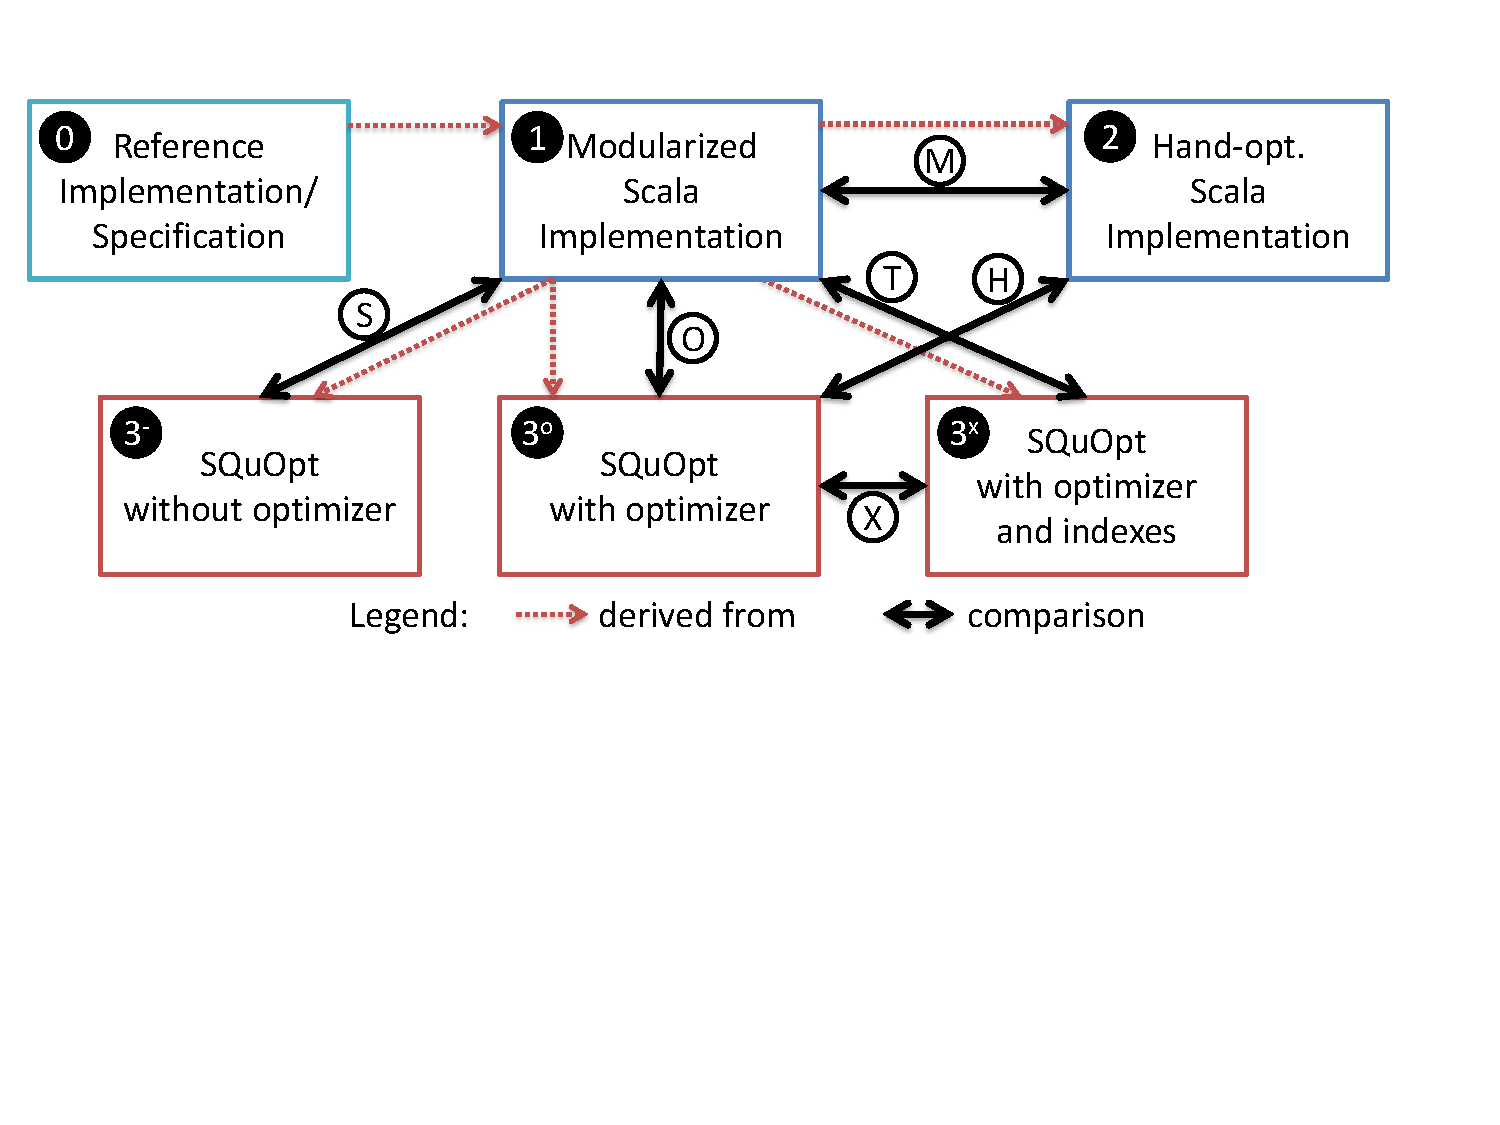
\includegraphics[width=\linewidth]{aosd13/graphs/measurements-overview}
	\caption{Measurement Setup: Overview}
	\label{fig:measurements-overview}
\end{figure}


\section{Experimental Units}




%selecting queries
%\begin{table*}
%\begin{tabular}{ll}\toprule
%Identifier & Description \\ \midrule
%PROTECTED\_FIELD % Findbugs: CI\_CONFUSED\_INHERITANCE
%%	& % Idealized: 4
%	& Class is final but declares protected field \\
%NO\_CLONE % Findbugs: CN\_IDOM
%%	& % Idealized: 9
%	&  Class implements Cloneable but does not define or use clone method \\
%SUPER\_CLONE\_MISSING % Findbugs: CN\_IDIOM\_NO\_SUPER\_CALL
%%	& % Idealized: 11
%	& The clone method does not call super.clone() \\
%NOT\_CLONEABLE % Findbugs: CN\_IMPLEMENTS\_CLONE\_BUT\_NOT\_CLONEABLE
%%	& % Idealized: 5
%	& Class defines clone() but doesn't implement Cloneable\\
%COVARIANT\_COMPARETO % Findbugs CO\_ABSTRACT\_SELF \& CO\_SELF\_NO\_OBJECT
%%	& % Idealized: 7
%	& Covariant compareTo() method defined\\
%GC\_CALL % Findbugs:  DM\_GC
%%	& % Idealized: 12
%	& Explicit garbage collection; extremely dubious except in benchmarking code\\
%RUN\_FINALIZERS\_ON\_EXIT % Findbugs DM\_RUN\_FINALIZERS\_ON\_EXIT
%%	& % Idealized: 12
%	& Method invokes dangerous method runFinalizersOnExit\\
%COVARIANT\_EQUALS %Findbugs: EQ\_ABSTRACT\_SELF
%%	& % Idealized: 4
%	& Abstract class defines covariant equals() method \\
%FINALIZER\_NOT\_PROTECTED % Findbugs: FI_PUBLIC_SHOULD_BE_PROTECTED
%%	& % Idealized: 6
%	& Finalizer should be protected, not public\\
%%NO\_SUITABLE\_CONSTRUCTOR% Findbugs: SE\_NO\_SUITABLE\_CONSTRUCTOR
%%	& % Idealized: 7
%%	& Class is Serializable but its superclass doesn't define a void constructor\\
%UNUSED\_PRIVATE\_FIELD % Findbugs: UUF\_UNUSED\_FIELD
%%	& % Idealized: 23
%	& The value of a private field is not read\\
%DONT\_CATCH\_IMSE  %Findbugs: IMSE\_DONT\_CATCH\_IMSE
%%	& % Idealized: 5
%	& Dubious catching of IllegalMonitorStateException \\\bottomrule
%\end{tabular}
%\nocaptionrule\caption{Implemented Analyses}
%\label{table:implemented-analyses}
%\end{table*}


\newcommand{\captionEvalTable}{%
As in in \cref{sec:implemenationsandspeedups}, (1) denotes the modular Scala
implementation, (2) the hand-optimized Scala one, and ($3^-$), ($3^o$), ($3^x$)
refer to the {\LoS} implementation when run, respectively, without
optimizations, with optimizations, with optimizations and indexing.
Queries marked with the $R$ superscript were selected by random sampling.}
\newcommand{\tablerowsize}{\scriptsize}
\begin{sidewaystable}[ph!]
\centering
\input{\graphPath{EvalTable}}
\nocaptionrule\caption{Performance results. \captionEvalTable}
\label{table:performance}
\end{sidewaystable}



\begin{table}[h]
  \centering
  \footnotesize
\input{\graphPath{EvalSummaryTable}}
\nocaptionrule\caption{Average performance ratios.
This table summarizes all interesting performance ratios across all queries,
using the geometric mean~\citep{Fleming86}.
The meaning of speedups is discussed in \cref{sec:implemenationsandspeedups}.}
\label{table:performanceAvg}
\end{table}

\begin{table}[h!]
\begin{tabular}{p{7cm}r}\toprule
Abstraction & Used \\ \midrule
% calculate class hierarchy & 5 \\
All fields in all class files	& 4\\
All methods in all class files	& 3\\
All method bodies in all class files	& 3\\
All instructions in all method bodies and their bytecode index	& 5\\
Sliding window (size $n$) over all instructions (and their index) &	3\\
\bottomrule
\end{tabular}\\
\nocaptionrule\caption{Description of abstractions removed during hand-optimization and number of queries where the abstraction is used (and optimized away).}
\label{table:implemented-abstractions}
\end{table}

\begin{extraEval}
\begin{table*}[tb]
\centering
\begin{tabular}{l*{3}{r@{}c@{}l}r*{2}{r@{}c@{}l}}\toprule
Name&\multicolumn{3}{c}{Base impl.\ (in ms)}&\multicolumn{3}{c}{Modular impl}&\multicolumn{3}{c}{Optimiz.\ time}&IS&\multicolumn{3}{c}{OS}&\multicolumn{3}{c}{OS-Opt}\\\midrule
\input{\graphPath{table}}
\bottomrule
\end{tabular}
\nocaptionrule\caption{Old performance results table}
\label{table:performanceOld}
\end{table*}
\end{extraEval}


As experimental units, we sampled a set of queries on code structures from FindBugs 2.0~\citep{DBLP:journals/sigplan/HovemeyerP04}. FindBugs is a popular bug-finding tool for Java Bytecode available as open source. To detect instances of bug patterns, it queries a structural in-memory representation of a code base (extracted from bytecode).
Concretely, a single loop traverses each class and invokes all visitors (implemented as listeners) on each element of the class. Many visitors, in turn, perform activities concerning multiple bug detectors which are fused together. An extreme example is that, in FindBugs, query \queryRUNFINALIZERSONEXIT{} is defined in class \code{DumbMethods} together with other 41 bug detectors for distinct types of bugs.
Typically a bug detector is furthermore scattered across the different methods of the visitor, which handle different elements of the class.
We believe this architecture has been chosen to achieve good performance; however, we do not consider such manual fusion of distinct bug detectors together as modular. We selected queries from FindBugs because they represent typical non-trivial queries on in-memory collections and because we believe our framework allows expressing them more modularly.

We sampled queries in two batches. First, we manually selected \manualQueryCount~queries (from approx.\ 400~queries in FindBugs), chosen mainly to evaluate the potential speedups of indexing (queries that primarily looked for declarations of classes, methods, or fields with specific properties, queries that inspect the type hierarchy, and queries that required analyzing methods implementation).
Subsequently, we \emph{randomly} selected a batch of \randomQueryCount~additional queries.
The batch excluded queries that rely on control-/dataflow analyses (i.e., analyzing the effect of bytecode instructions on the stack), due to limitations of the bytecode tookit we use.
In total, we have \queryCount{} queries as listed in \cref{table:performance} (the randomly selected queries are marked with the superscript $R$).




%Omit - this only showcases BAT, not our code. Show our implementation instead.
\begin{figure}[htb]
\centering
%\begin{lstlisting}
%for {
%  cf <- classFiles
%  m @ Method(_, "equals", MethodDescriptor(Seq(cf.thisClass), BooleanType), _) <- cf.methods
%  if m.isAbstract
%} yield (cf, m)
%\end{lstlisting}
%import BATLifting._
\begin{lstlisting}
for {
  classFile <- classFiles.asSquopt
  method <- classFile.methods
  if method.isAbstract && method.name ==# "equals" &&
     method.descriptor.returnType ==# BooleanType
  parameterTypes <- Let(method.descriptor.parameterTypes)
  if parameterTypes.length ==# 1 &&
     parameterTypes(0) ==# classFile.thisClass
} yield (classFile, method)
\end{lstlisting}
\caption{Find covariant \code{equals} methods.}
\label{fig:covariant-equals}
\end{figure}



%reimplementation
We implemented each query three times (see implementations (1)--(3) in \cref{sec:implemenationsandspeedups}) following the specifications given in the FindBugs documentation (0). Instead of using a hierarchy of visitors as the original implementations of the queries in FindBugs, we wrote the queries as for-comprehensions in Scala on an in-memory representation created by the Scala toolkit BAT\@.\footnote{\url{http://github.com/Delors/BAT}}
BAT in particular provides comprehensive support for
writing queries against Java bytecode in an idiomatic way.
We exemplify an analysis in \cref{fig:covariant-equals}: It detects all co-variant \code{equals} methods in a project by iterating over all class files (line 2) and all methods, searching for methods named ``\code{equals}'' that return a boolean value and define a single parameter of the type of the current class.


\smartParagraph{Abstractions}
In the reference implementations (1), we identified several reusable abstractions as shown in \cref{table:implemented-abstractions}.
The reference implementations of all queries except \querySEBADFIELDINNERCLASS{} use exactly one of these abstractions, which encapsulate the main loops of the queries.

\smartParagraph{Indexes}
For executing ($3^x$) (\LoS\ with indexes), we have constructed three indexes to speed up navigation over the queried data of queries 1--\manualQueryCount{}: Indexes for method name, exception handlers, and instruction types. We illustrate the implementation of the method-name index in \cref{fig:indexes}: it produces a collection of all methods and then indexes them using \code{indexBy}; its argument extracts from an entry the key, that is the method name.
We selected which indexes to implement using guidance from \LoS{} itself; during optimizations, \LoS{} reports which indexes it could have applied to the given query. Among those, we tried to select indexes giving a reasonable compromise between construction cost and optimization speedup.
%% If we want to show the raw data, we could use this LaTeX code - but we need updated, and correct, data!
We first measured the construction cost of these indexes:

\begin{center}
\begin{tabular}{l*{1}{r@{}c@{}l}}\toprule
Index&\multicolumn{3}{c}{Elapsed time (ms)}\\\midrule

Method name&$97.99$&$\pm$&$2.94$\\
Exception handlers&$179.29$&$\pm$&$3.21$\\
Instruction type&$4166.49$&$\pm$&$202.85$\\

\bottomrule
\end{tabular}
\end{center}
For our test data, index construction takes less than 200 ms for the first two indexes, which is moderate compared to the time for loading the bytecode in the BAT representation ($\readingClassFilesTime$). Building the instruction index took around 4 seconds, which we consider acceptable since this index maps each type of instruction (e.g.\ \code{INSTANCEOF}) to a collection of all bytecode instructions of that type.
%Valid question: why does the exception-handler index take so much more than the query it optimizes? That's because indexes are interpreted. But it's best not to say it. Also, we already discuss this later convincingly.

%The first index maps any method name to the corresponding methods (together with containing classes), and is used by many different queries. Its implementation is shown in \cref{fig:indexes}: the code shown first produces a collection of all methods and then indexes them using \code{indexBy}; its argument extracts from an entry the key, that is the method name.
%The second index maps any exception type to exception handlers catching them (together with the containing method bodies, methods and class).
%The third index allows to look for occurrences of bytecode instructions of a given type; it maps any type of bytecode instruction (like \code{INVOKESTATIC}, \code{INVOKEVIRTUAL} and so on) to its occurrences.

\begin{figure}
\centering
\begin{lstlisting}
val methodNameIdx: Exp[Map[String, Seq[(ClassFile, Method)]]] = (for {
  classFile <- classFiles.asSquopt
  method <- classFile.methods
} yield (classFile, method)).indexBy(entry => entry._2.name)
\end{lstlisting}
\caption{A simple index definition}
\label{fig:indexes}
\end{figure}



\section{Measurement Setup}
To measure performance, we executed the queries on the preinstalled JDK class library (\texttt{rt.jar}), containing 58M of uncompressed Java bytecode.
We also performed a preliminary evaluation by running queries on the much smaller ScalaTest library, getting comparable results that we hence do not discuss.
Experiments were run on a 8-core Intel Core i7-2600, 3.40 GHz, with 8 GB of RAM, running Scientific Linux release 6.2.
The benchmark code itself is single-threaded, so it uses only one core; however the JVM used also other cores to offload garbage collection.
We used the preinstalled OpenJDK Java version 1.7.0\_05-icedtea and Scala 2.10.0-M7.

We measure steady-state performance as recommended by \citet{Georges07rigorousJavaPerformance}. We invoke the JVM $p = 15$ times;
at the beginning of each JVM invocation, all the bytecode to analyze is loaded in memory and converted into BAT's representation.
In each JVM invocation, we iterate each benchmark until the variations of results becomes low enough. We measure the variations of results through the coefficient of variation (CoV; standard deviation divided by the mean). Thus, we iterate each benchmark until the CoV in the last $k = \kZrememberedSampleLoops$ iterations drops under the threshold $\theta = \thetaZmaxCov$, or until we complete $q = \qZmaxLoops$ iterations.
We report the arithmetic mean of these measurements (and also report the usually low standard deviation on our web page).
%PG: I had p = 3, k = 50, theta = 0.02, q = 1000, but changed the parameters when running more queries.

\section{Results}

\smartParagraph{Correctness} We machine-checked that for each query, all variants in \cref{table:performance} agree.

\smartParagraph{Modularization Overhead}
We first observe that performance suffers significantly when using the abstractions we described in \cref{table:implemented-abstractions}. These abstractions, while natural in the domain and in the setting of a declarative language, are not idiomatic in Java or Scala because, without optimization, they
will obviously lead to bad performance. They are still useful abstractions from the point of view of modularity, though---as indicated by \cref{table:implemented-abstractions}---and as such it would be desirable if one could use them without paying the performance penalty.


\smartParagraph{Scala Implementations vs.\ FindBugs}
Before actually comparing between the different Scala and \LoS\ implementations, we first ensured that the implementations are comparable to the original FindBugs implementation. A direct comparison between the FindBugs reference implementation and any of our implementations is not possible in a rigorous and fair manner. FindBugs bug detectors are not fully modularized, therefore we cannot reasonably isolate the implementation of the selected queries from support code. Furthermore, the architecture of the implementation has many differences that affect performance: among others, FindBugs also uses multithreading. Moreover, while in our case each query loops over all classes, in FindBugs, as discussed above, a single loop considers each class and invokes all visitors (implemented as listeners) on it.

We measured \emph{startup performance}~\citep{Georges07rigorousJavaPerformance}, that is the performance of running the queries only once, to minimize the effect of compiler optimizations.
We setup our \LoS-based analyses to only perform optimization and run the optimized query. To setup FindBugs, we manually disabled all unrelated bug detectors; we also made the modified FindBugs source code available. The result is that the performance of the Scala implementations of the queries ($3^-$) has performance of the same order of magnitude as the original FindBugs queries -- in our tests, the \LoS\ implementation was about twice as fast. However, since the comparison cannot be made fair, we refrained from a more detailed investigation.

% XXX HACK
\smartParagraph{SQuOpt Overhead and Optimization Potential}
We present the results of our benchmarks in \cref{table:performance}.
Column names refer to a few of the definitions described above; for readability, we do not present all the ratios previously introduced for each query, but report the raw data.
In \cref{table:performanceAvg}, we report the geometric mean \cite{Fleming86} of each ratio, computed with the same weight for each query.

%queries are between \maxInterpOver{}x slower and \maxInvInterpOver{}x faster; on average \LoS\ queries are \geoMeanInvInterpOver{}x faster.
%\minInvInterpOver{}x and \maxInvInterpOver{}x---that is, queries are between \minInterpOver{}x and
We see that, in its current implementation, \LoS\ can cause a overhead S
(1/$3^-$) up to \maxInterpOver{}x. On average \LoS\ queries are
\geoMeanInterpOver{}x faster. These differences are due to minor implementation
details of certain collection operators.
For query $18^R$, instead, we have that the the basic \LoS\ implementation is \maxInvInterpOver{}x faster and are investigating the reason; we suspect this might be related to the use of pattern matching in the original query.

As expected, not all queries benefit from optimizations;
out of \queryCount{} queries, optimization affords for \nSpeededUpQueries{} of them significant speedups ranging from a \minOptimSpeedup{} factor to a \maxOptimSpeedup{} factor; \nBigSpeededUpQueries{} queries are faster by a factor of at least \speedupBigThreshold{}.
Only queries \queryMSPKGPROTECT{}, \querySICINNERSHOULDBESTATICANON{} and \queryITAINEFFICIENTTOARRAY{} fail to recover any modularization overhead.

We have analyzed the behavior of a few queries after optimization, to understand why their performance has
(or has not) improved.

Optimization makes query \querySEBADFIELDINNERCLASS{} slower; we believe this is because optimization replaces filtering by lazy filtering, which is usually faster, but not here.
Among queries where indexing succeeds, query \queryGCCALL{} has the least speedup. After optimization, this query uses the instruction-type index to find all occurrences of invocation opcodes (\code{INVOKESTATIC} and \code{INVOKEVIRTUAL}); after this step the query looks, among those invocations, for ones targeting \code{runFinalizersOnExit}. Since invocation opcodes are quite frequent, the used index is not very specific, hence it allows for little speedup (\speedupTGCCALL). However no other index applies to this query; moreover, our framework does not maintain any selectivity statistics on indexes to predict these effects.
Query \queryFIUSELESS{} benefits from indexing without any specific tuning on our part, because it looks for implementations of \code{finalize} with some characteristic, hence the highly selective method-name index applies.
After optimization, query \queryDONTCATCHIMSE{} becomes simply an index lookup on the index for exception handlers, looking for handlers of \code{IllegalMonitorStateException}; it is thus not surprising that its speedup is thus extremely high (\maxOptimSpeedup{}). This speedup relies on an index which is specific for this kind of query, and building this index is slower than executing the unoptimized query. On the other hand, building this index is entirely appropriate in a situation where similar queries are common enough. Similar considerations apply to usage of indexing in general, similarly to what happens in databases.

\smartParagraph{Optimization Overhead}
The current implementation of the optimizer is not yet optimized for speed (of the optimization algorithm). For instance, expression trees are traversed and rebuilt completely once for each transformation.
However, the optimization overhead is usually not excessive and
is $\avgOptimTime \pm \stdDevOptimTime$ ms, varying between \minOptimTime{} ms and \maxOptimTime{} ms (mostly depending on the query size).

\smartParagraph{Limitations}
Although many speedups are encouraging, our optimizer is currently a proof-of-concept and we experienced some limitations:
\begin{itemize}
\item In a few cases hand-optimized queries are still faster than what the optimizer can produce. We believe these problems could be addressed by adding further optimizations.
\item Our implementation of indexing is currently limited to immutable collections. For mutable collections, indexes must be maintained incrementally.
Since indexes are defined as special queries in {\LoS},  incremental index maintenance becomes an instance of incremental maintenance of query results, that is, of incremental view maintenance. We plan to support incremental view maintenance as part of future work; however,
indexing in the current form is already useful, as illustrated by our experimental results.
\end{itemize}

\smartParagraph{Threats to Validity}
With rigorous performance measurements and the chosen setup, our study was setup to maximize internal and construct validity. Although we did not involve an external domain expert and we did not compare the results of our queries with the ones from FindBugs (except while developing the queries), we believe that the queries adequately represent the modularity and performance characteristics of FindBugs and {\LoS}. However, since we selected only queries from a single project, external validity is limited.
While we cannot generalize our results beyond FindBugs yet, we believe that the FindBugs queries are representative for complex in-memory queries performed by applications.


\smartParagraph{Summary}
We demonstrated on our real-world queries that relying on declarative abstractions in collection queries often causes a significant slowdown. As we have seen, using \LoS\ without optimization, or when no optimizations are possible, usually provides performance comparable to using standard Scala; however, \LoS\ optimizations can in most cases remove the slowdown due to declarative abstractions. Furthermore, relying on indexing allows to achieve even greater speedups while still using a declarative programming style.
Some implementation limitations restrict the effectiveness of our optimizer, but since this is a preliminary implementation, we believe our evaluation shows the great potential of optimizing queries to in-memory collections.


% vim: set tw=0:



\chapter{Discussion}
\label{ch:aosd13-discussion}
\label{sec:discussion}
In this chapter we discuss the degree to which \LoS\ fulfilled our original design goals, and the conclusions
for host and domain-specific language design.

\section{Optimization limitations}
\label{sec:optim-vs-inc}
In our experiments indexing achieved significant speedups, but when indexing
does not apply speedups are more limited; in comparison, later projects working
on collection query optimization, such as OptiQL~\citep{Rompf13,Arvind13}, gave
better speedups, as also discussed in \cref{sec:rwdsl-lms}.

A design goal of this project was to incrementalize optimized queries, and while
it is easy to incrementalize collection operators such as \texttt{map},
\texttt{flatMap} or \texttt{filter}, it was much less clear to us how to
optimize the result of inlining.
We considered using shortcut fusion, but we did
not know a good way to incrementalize the resulting programs; later work, as
described in \cref{part:incr}, clarified what is possible and what not.

Another problem is that most fusion techniques are designed for sequential
processing, hence conflict with incrementalization.
Most fusion techniques generally assume bulk operations scan collections in
linear order. For instance, shortcut fusion rewrites operators in terms of
\texttt{foldr}.
During parallel and/or incremental computation, instead, it is better to use
\emph{tree-shaped folds}: that is, to split the task in a divide-and-conquer
fashion, so that the various subproblems form a balanced tree. This division
minimizes the height of the tree, hence the number of steps needed to combine
results from subproblems into the final result, as also discussed by
\citet{Steele2009organizing}. It is not so clear how to apply shortcut fusion to
parallel and incremental programs.
\citet{Maier2013} describe an incremental tree-shaped fold, where each
subproblem that is small enough is solved by scanning its input in linear order,
but does not perform code transformation and does not study how to perform fusion.

\section{Deep embedding}
\subsection{What worked well}
Several features of Scala contributed greatly to the success we achieved. With implicit conversions, the lifting can be made mostly transparent. The advanced type system features were quite helpful to make the expression tree representation typed. The fact that for-comprehensions are desugared \emph{before} type inference and type checking was also a prerequisite for automatic lifting. The syntactic expressiveness and uniformity of Scala, in particular the fact that custom types can have the same look-and-feel as primitive types, were also vital to lift expressions on primitive types.

%\subsection{What did not work so well; limitations}
\subsection{Limitations}
\label{sec:limitations}
Despite these positive experiences and our experimental success, our embedding has a few significant limitations.

The first limitation is that we only lift a subset of Scala, and some interesting features are missing.
We do not support \emph{statements} in nested blocks in our queries, but this could be implemented reusing techniques from Delite~\citep{Rompf11BBlocks}.
%\smartParagraph{Virtualized pattern matching}
More importantly for queries, \emph{pattern matching} cannot be supported by deep embedding similar to ours. In contrast to for-comprehension syntax, pattern matching is desugared only \emph{after} type checking \cite{Emir07Patterns}, which prevents us from lifting pattern matching notation. More specifically, because an extractor \cite{Emir07Patterns} cannot return the representation of a result value (say \code{Exp[Boolean]}) to later evaluate; it must produce its final result at pattern matching time. There is initial work on ``virtualized pattern matching''\footnote{\url{http://stackoverflow.com/questions/8533826/what-is-scalas-experimental-virtual-pattern-matcher}}, and we hope to use this feature in future work.

We also experienced problems with operators that cannot be overloaded, such as \code{==} or \code{if-else} and with lifting methods in \code{scala.Any}, which forced us to provide alternative syntax for these features in queries. The  Scala-virtualized project \citep{Moors12Virtualized} aims to address these limitations; unfortunately, it advertises no change on the other problems we found, which we subsequently detail.

%Pattern matching cannot be virtualized as-is,

It would also be desirable if we could enforce the absence of side effects in queries, but since Scala, like most practical programming languages except Haskell, does not track side effects in the type system this does not seem to be possible.
%However, we believe that the advantages of purely functional queries are a more desirable interface.

Finally, compared to \emph{lightweight modular staging}~\citep{rompf2010lightweight} (the foundation of Delite) and to polymorphic embedding~\citep{hofer08polymorphic}, we have less static checking for some programming errors when writing queries; the recommended way to use Delite is to write a EDSL program in one trait, in terms of the EDSL interface only, and combine it with the implementation in another trait. In polymorphic embedding, the EDSL program is a function of the specific implementation (in this case, semantics).
Either approach ensures that the DSL program is \emph{parametric} in the implementation, and hence cannot refer to details of a specific implementation.
However, we judged the syntactic overhead for the programmer to be too high to use those techniques -- in our implementation we rely on encapsulation and on dynamic checks at query construction time to achieve similar guarantees.

The choice of interpreting expressions turned out to be a significant performance limitation. It could likely be addressed by using Delite and lightweight modular staging instead, but we wanted to experiment with how far we can get \emph{within} the language in a well-typed setting.

%The first is
%\pg{We don't support pattern matching in the user interface.}

\subsection{What did not work so well: Scala type inference}
\label{sec:ScalaLessons}

%\pg{Continue:
%When implementing our library, we often struggled against limitations and bugs in the Scala compiler, especially regarding type inference and its interaction with implicit resolution. Scala's type inference is not complete.
%%, hence it does not guarantee
%%When using implicit conversions to encode
%}
%\pg{Examples: nested constructors; shadowing of functions; pattern matching in the optimizer}.
%\pg{Our expression trees are only partially typed - discuss limitations of the optimizer.}
%
%\pg{as soon as we try supporting nesting tuples such as \code{((a, b), c}, we face again type inference bugs, for which this time we found no reasonable workaround which does not affect surface syntax. The conversion above accepts a pair of expression trees; we can write a more general conversion which accepts a pair of values \emph{implicitly convertible} to expression trees, so that \code{asExp((a, b), c)} would have type \code{Exp[((A, B), C)]}, but the compiler cannot make use of this conversion\footnote{We reported \url{https://issues.scala-lang.org/browse/SI-5651}, probably a dup of \url{https://issues.scala-lang.org/browse/SI-3346}.}}.
%
%
%\pg{Discuss that type inference constrains library design.}

%\pg{Move discussion of type inference to the discussion Section}
%%However, Scala only features \emph{local} type inference; one often needs to consider the type inference algorithm when writing method signatures, especially for higher-order methods, to ensure that the client code does not need redundant type annotations.
%
%Since \code{map} is part of the collection EDSL, and since for-comprehensions are desugared to expressions using \code{map}, we need to lift this method carefully. Clients should not need extra type annotations for using the lifted version; moreover, we want to receive a reified version of the parameter.
%
%%one can often write type signatures to ensure that it works.
%
%In this example, type inference can consider the type of \code{map}, unify \code{T} with \code{String} and \code{T => U} with the type of \code{str => str + "!"}. Type inference deduces that \code{str} must also have type \code{T = String}, and can then typecheck the function body and deduce that its return type, \code{U}, is also \code{String}.


%\pg{The interpretation overhead is higher than we expected, both with and without HOAS; maybe better JIT compilers could help?}
%\pg{We do not reject inadequate object programs at compile time, but only when queries are built.}


%\pg{One of the additional goal was to have our optimization work within the language visible to the user. We didn't succeed so much, for various reasons; on the other hand, this seems orthogonal to the meta-goals of the paper, and our failure does not seem to be insightful.}

%In our optimizer, we initially wanted to keep the language quite close to the user language. That however was not possible.
%We plan reusing different approaches to query optimization, based on monoid homomorphisms. On the other hand, different semantics might require the original language structure.

%% Collections interface.
%\smartParagraph{Limitations and discussion.}
%
%However, instead of just lifting those methods from \code{TraversableLike}, we modified them slightly. These differences, however, do not limit the ability to write queries with our framework, as we will illustrate.\pg{Any supporting evidence?}
%This is not due to a limitation of our approach; we experimented with lifting the original signatures faithfully, but in the end abandoned this attempt because of opposing design goals for the interface of our EDSL:
%\begin{itemize}
%\item expressions in the Scala collections EDSL have an accurate static type, and we want to preserve that accuracy by making the lifting as faithful as possible;
%\item we want our expression trees to support different semantics reasonably well, including interpretation and optimization.
%\item we want to minimize the amount of code we need, and have minimal coupling to the collection library. For instance, the framework should support new implementation of dictionaries with as few changes as possible to the framework.
%\end{itemize}
%Furthermore, an additional non-functional constraint is that we need an interface which type inference understands.
%
%These three goals are opposing and we cannot reach all of them at the same time. In the end, we make the following choices.
%\begin{itemize}
%%\item We only support purely functional interfaces, to simplify optimizations. \pg{Probably comment this out, already said.}
%\item We only support \code{Traversable[T]} and its subtypes. Some optimizations are unsafe for more generic collection types.
%For instance, we do not support iterators (whose interface relies on side effects), nor do we support \code{FilterMonadic[T, Repr]}.
%Additionally, this excludes support for parallel collections, which is left however for future work.
%\item For instance, we want to have just a single type of node to represent \code{flatMap} operations, and not a different one for each kind of collection, hence we lift \code{TraversableLike}. On the other hand, to make our optimizations safe, we only consider collections which are subtype of \code{Traversable[T]}. As a consequence, \code{withFilter} returns the representation of a new concrete collection, instead of a proxy of type \code{Exp[FilterMonadic[T, Repr]]}, and thus has the semantics of \code{filter}; the two semantics are however indistinguishable at run time in absence of side effects.
%Moreover, restricting to subtype of \code{Traversable[T]} implies excluding iterators, which however lack a purely functional interface; support for parallel collections instead is left as future work.
%\item We currently only support a subset of methods (only the ones we ever needed), to be able to provide different semantics more easily.
%\end{itemize}

%%% implicit conversions
%However, with the definitions so far, expressions such as \code{"bar" + x} cannot yet be lifted. To make this expression typecheck, the compiler should transform it to
%\code{expToStringOps(pure("bar")) + x} by chaining two implicit conversions. However, the rules for implicit conversions in Scala explicitly disallow this transformation, to avoid different implicit conversions to chain in unintended ways.

%\citet[Ch.~21]{Odersky11book} explain how one can selectively allow chaining of implicit conversions.
%We could modify \code{expToStringOps(Exp[String])} to accept any parameter which can be converted to \code{Exp[String]}, together with
%such an implicit conversion, as follows:
%\begin{lstlisting}
%implicit def expToStringOps[T](x: T)
%    (implicit conv: T => Exp[String]) =
%    new StringOps(conv(x))
%\end{lstlisting}
%However, this does not work due to hard-to-fix bugs in Scala type inference\footnote{The problem is demonstrated at \url{https://gist.github.com/2146097}; the bug report is available at \url{https://issues.scala-lang.org/browse/SI-3346}.}.
%Hence we need to write a new implicit conversion, chaining those two conversions explicitly:
%
%\begin{lstlisting}
%implicit def toStringOps(t: String) = expToStringOps(pure(t))
%\end{lstlisting}


%\smartParagraph{Functions}
%Functions can be lifted similarly to methods. For a function \code{f} with parameter types \code{A1}, \ldots, \code{An} and result type \code{R}, one can provide an overload of \code{f} with parameter types \code{Exp[A1]}, \ldots, \code{Exp[An]} and result type \code{Exp[R]} which creates an expression node representing the function call.
%This also extends to constructors of case classes, like \code{BookData} in the examples above. However, this function shadows the original one. While the ambiguity could be resolved by overload resolution, it is not, hence we need to import the new function only in a restricted scope.
%\pg{Should I say more here?}
%
%\smartParagraph{Implicit conversions}
%We also need to lift implicit conversions: Whenever values of type \code{T} can be converted to type \code{U}, we want that also values of type \code{Exp[T]} can be converted to type \code{Exp[U]}, to keep the behavior of lifted code similar. We can do so similarly to how we lift a function, but since implicit names do not appear in user code normally, we can choose a different name and avoid shadowing problems.
%
%\pg{Should I say more here?}

%The following implicit conversion should be enough to lift at once all implicit conversions:
%\begin{lstlisting}
%implicit def liftConv[T, U](t: Exp[T])(implicit conv: T => U): Exp[U] = //...
%\end{lstlisting}
%However, the Scala compiler is not able to use this implicit conversion, for unclear reasons (we believe because of some type inference bug).
%Hence for each implicit conversion we need to define a lifting.
%\pg{This and the previous ones are bugs which I could workaround rather easily; later I have a bug which I cannot workaround.}

% I wanted to show this code, which does run into a known bug, but it does not do the right thing.
%\begin{lstlisting}
%implicit def pure[T, U <% T](t: U): Exp[T] = Const(t)
%\end{lstlisting}

%One such context is:
%\begin{lstlisting}
%def asExp[T](t: Exp[T]) = t
%\end{lstlisting}
%Note that \code{asExp} is an identity function, but restricted to expression trees; this triggers the Scala compiler to use an implicit resolution if needed. Standard rules for implicit resolution apply, which select the implicit conversion with the most specific type. Hence, while \code{pure((a, b))} would produce \code{Const((a, b))} with type \code{Exp[(Exp[A], Exp[B])]},
%\code{asExp((a, b))} produces \code{LiftTuple2(a, b)} with type \code{Exp[(A, B)]}, that is a representation of \code{(a, b)}, as desired.
%
%
%\pg{Actually, the problem shows up with any two nested constructors of this kind.}
%
%EDSL programs need to resort to calling \code{asExp} extremely rarely, because operations of the EDSL already provide the needed context; but as soon as we try supporting nesting tuples such as \code{((a, b), c}, we face again type inference bugs, for which this time we found no reasonable workaround which does not affect surface syntax. The conversion above accepts a pair of expression trees; we can write a more general conversion which accepts a pair of values \emph{implicitly convertible} to expression trees, so that \code{asExp((a, b), c)} would have type \code{Exp[((A, B), C)]}, but the compiler cannot make use of this conversion\footnote{We reported \url{https://issues.scala-lang.org/browse/SI-5651}, probably a dup of \url{https://issues.scala-lang.org/browse/SI-3346}.}.
%The problem generalizes to any two nested generic constructors.
%
%We observe that these limitations of type inference make its behavior hard to predict and hinder DSL embedding. We discuss this point further in \cref{sec:ScalaLessons}.


%\subsubsection{Lessons about Scala}
%\pg{Make the line of thought explicit.}
When implementing our library, we often struggled against limitations and bugs in the Scala compiler, especially regarding type inference and its interaction with implicit resolution, and we were often constrained by its limitations. Not only Scala's type inference is not complete, but we learned that its behavior is only specified by the behavior of the current implementation: in many cases where there is a clear desirable solution, type inference fails or finds an incorrect substitution which leads to a type error. Hence we cannot distinguish, in the discussion, the Scala language from its implementation.
We regard many of Scala's type inference problems as bugs, and reported them as such when no previous bug report existed, as noted in the rest of this section. Some of them are long-standing issues, others of them were accepted, for other ones we received no feedback yet at the time of this writing, and another one was already closed as WONTFIX, indicating that a fix would be possible but have excessive complexity for the time being.\footnote{\url{https://issues.scala-lang.org/browse/SI-2551}}

\smartParagraph{Overloading}
The code in Fig.~\ref{fig:reifiedQuery} uses the lifted \code{BookData} constructor. Two definitions of \code{BookData} are available, with signatures \code{BookData(String, String, Int)} and \code{BookData(Exp[String],}\linebreak\code{Exp[String], Exp[Int])}, and it seems like the Scala compiler should be able to choose which one to apply using overload resolution. This however is not supported simply because the two functions are defined in different scopes,\footnote{\url{https://issues.scala-lang.org/browse/SI-2551}} hence importing \code{BookData(Exp[String], Exp[String], Exp[Int])} shadows locally the original definition.
%\pg{Resume}
% function of type \code{}
% are reported as bugs; some of them were already acknowledged, others were found to be already known.
%During our work we reported many of the bugs we found; we provide links to the ones which are still not addressed and which support
%\pg{Say something about bugs found.}

%defined
%apparently the only description of its behavior

%We found various limitations of type inference for Scala.
%Note that we identify the language and its implementation in the following, since type inference is not specified, hence Scala's type inference is de facto specified by its only implementation.

\smartParagraph{Type inference vs implicit resolution}
The interaction between type inference and implicit resolution is a hard problem, and Scalac has also many bugs, but the current situation requires further research; for instance, there is not even a specification for the behavior of type inference\footnote{\url{https://issues.scala-lang.org/browse/SI-5298?focusedCommentId=55971##comment-55971}, reported by us.}.

As a consequence, to the best of our knowledge some properties of type inference have not been formally established.
For instance, a reasonable user expectation is that removing a call to an implicit conversion does not alter the program, if it is the only implicit conversion with the correct type in scope, or if it is more specific than the others~\citep[Ch.~21]{Odersky11book}. This is not always correct, because removing the implicit conversion reduces the information available for the type inference algorithm; we observed multiple cases\footnote{\url{https://issues.scala-lang.org/browse/SI-5592}, reported by us.} where type inference becomes unable to figure out enough information about the type to trigger implicit conversion.

We also consider significant that Scala 2.8 required making both type inference and implicit resolution more powerful, specifically in order to support the collection library~\citep[Sec.~21.7]{Moors10TCP,Odersky11book}; further extensions would be possible and desirable.
For instance, if type inference were extended with higher-order unification\footnote{\url{https://issues.scala-lang.org/browse/SI-2712}}~\citep{Pfenning88}, it would better support a part of our DSL interface (not discussed in this chapter) by removing the need for type annotations.
%\pg{That's type indexing, to describe earlier}.

%We believe that as long as such problems are addressed in a ad-hoc way, users will be at a disadvantage in their ability to \emph{grow their language} in a seamless way~\citep{Steele99Growing}. \pg{This sounds cool, should go to the conclusions.}
% See commit d66fec6d4081ebf3a34a766f6c8203199c1c6f1f and Lifting.groupBySelImpl, add a bug report with these examples.

%Additionally, overloading is a second-class citizen in Scala - as long as it is there, one needs some support for it.
%It is also required to use it in some cases!

\smartParagraph{Nested pattern matches for GADTs in Scala}
Writing a typed decomposition for \code{Exp} requires pattern-matching support for generalized algebraic datatypes (GADTs). We found that support for GADTs in Scala is currently insufficient. \citet{Emir07Patterns} define the concept of \emph{typecasing}, essentially a form of pattern-matching limited to non-nested patterns, and demonstrate that Scala supports typecasing on GADTs in Scala by demonstrating a typed evaluator; however, typecasing is rather verbose for deep patterns, since one has to nest multiple pattern-matching expressions.
When using normal pattern matches, instead, the support for GADT seems much weaker.\footnote{Due to bug \url{https://issues.scala-lang.org/browse/SI-5298?focusedCommentId=56840##comment-56840}, reported by us.}
% seems hard to get the same level of support.
Hence one has to choose between support for GADT and the convenience of nested pattern matching.
A third alternative is to ignore or disable compiler warnings, but we did not consider this option. \pg{I would add that: ``Apparently this was instead the option chosen for Scala-virtualized~\citep{Moors12Virtualized}'', but I'd like to ask Adriaan first.}

% Should we write that it still does not work? No; I found no bug in the example which does not work, but a problem with the case class I wrote.

% XXX in fact, I now managed to prove manually something that the compiler does not get.

%It works to some extent, but only if the GADT does not use parametrized types, that is if generics are not involved. When generics are involved, erasure kicks in; moreover, one would often need to write non-linear type patterns, because the GADT definition implies different types to be equal.
%Finally, if I write two conditions on the same value in a pattern match, the typing refinement from one does not extend to the other (which correctly follows from the language definition). This however makes it impossible to nest multiple patterns.
%\pg{We tested with -unchecked warnings enabled - Scala-virtualized-tutorial disables this flag to shut up the warnings.}

% Ask Tillmann. That's somewhat true, but it's extremely hard to argue.
%The type-class pattern: in Haskell type-class resolution cannot happen locally inside a generic function; in Scala instead it can, even if for some instantiations a more precise instance might be available. This can lead to imprecise types, unless the programmer carefully figures out the implicit parameter which it needs to accept.

\smartParagraph{Implicit conversions do not chain}
While implicit conversions by default do not chain, it is sometimes convenient to allow chaining selectively.
For instance, let us assume a context such that \code{a: Exp[A]}, \code{b: Exp[B]} and \code{c: Exp[C]}.
In this context, let us consider again how we lift tuples. We have seen that the expression \code{(a, b)} has type \code{(Exp[A], Exp[B])} but can be converted to \code{Exp[(A, B)]} through an implicit conversion. Let us now consider \emph{nested} tuples, like \code{((a, b), c)}: it has type \code{((Exp[A], Exp[B]), Exp[C])}, hence the previous conversion cannot be applied to this expression.

\citet[Ch.~21]{Odersky11book} describe a pattern which can address this goal. Using this pattern, to lift pairs, we must write an implicit conversion from pairs of elements which can be \emph{implicitly converted} to expressions. Instead of requiring
\code{(Exp[A], Exp[B])}, the implicit conversion should require \code{(A, B)} with the condition that \code{A} can be converted to \code{Exp[A']} and \code{B} to \code{Exp[B']}. This conversion solves the problem if applied explicitly,
but the compiler refuses to apply it implicitly, again because of type inference issues\footnote{\url{https://issues.scala-lang.org/browse/SI-5651}, reported by us.}.

Because of these type inference limitations, we failed to provide support for reifying code like \code{((a, b), c)}\footnote{One could of course write a specific implicit conversions for \emph{this} case; however, \code{(a, (b, c))} requires already a different implicit conversion, and there are infinite ways to nest pairs, let alone tuples of bounded arity.}.
%Hence, we did not find a way to support nested tuples like

%For instance
%but as soon as we try supporting nesting tuples such as \code{((a, b), c},
%we face again type inference bugs, for which this time we found no reasonable workaround which does not affect surface syntax.

%having implicit parameters.
%\code{Exp[((A, B), C)]}

%The implicit conversion we described accepts a pair of expression trees; we can write a more general conversion which accepts a pair of values \emph{implicitly convertible} to expression trees, so that \code{asExp((a, b), c)} would have type \code{Exp[((A, B), C)]}, but the compiler cannot make use of this conversion\footnote{\url{https://issues.scala-lang.org/browse/SI-5651}, reported by us.}.
%
%%to selectively allow chaining of implicit conversions.
%
%An implicit conversion can request another one as parameter
%\pg{but that often does not work (again) because of issues with type inference.}
%The problem generalizes to any two nested generic constructors.


\smartParagraph{Error messages for implicit conversions}
The enrich-my-library pattern has the declared goal to allow to extend existing libraries \emph{transparently}. However, implementation details shine however through when a user program using this feature contains a type error. When invoking a method would require an implicit conversion which is not applicable, the compiler often just reports that the method is not available. The recommended approach to debugging such errors is to manually add the missing implicit conversion and investigating the type error~\citep[Ch.~21.8]{Odersky11book}, but this destroys the transparency of the approach when creating or modifying code.
\pg{Is our suggestion helpful? Is our complaint helpful without the suggestion?} We believe this could be solved in principle by research on error reporting: the compiler could automatically insert all implicit conversions enabling the method calls and report corresponding errors, even if at some performance cost.
%In principle, this same step could be performed by the compiler automatically to improve error reporting,


%Pimped methods are distinct from built-in methods, and the distinction is often too apparent.

\subsection{Lessons for language embedders}
Various domains, such as the one considered in our case study, allow powerful domain-specific optimizations. Such optimizations often are hard to express in a compositional way, hence they cannot be performed while building the query but must be expressed as global optimizations passes.
For those domains, deep embedding is key to allow significant optimizations.
%\footnote{The alert reader knows that any function on an inductive data type can be made compositional by representing more of the input in the output, but later this extra content must be removed anyway.}
On the other hand, deep embedding requires to implement an interpreter or a compiler.

On the one hand, interpretation overhead is significant in Scala, even when
using HOAS to take advantage of the metalevel implementation of argument access.
%Even when using an interpreter, however, the overhead can be compensated by the benefits for the user of the EDSL, which can write more declarative and modular queries, without paying an excessive cost because of interpretation.
%However, we believe that domain-specific optimizations enable the benefits for modularity are significant.

Instead of interpreting a program, one can compile a EDSL program to Scala and load it, as done by \citet{Rompf11BBlocks};
while we are using this approach, the disadvantage is the compilation delay,
especially for Scala whose compilation process is complex and time-consuming.
Possible alternatives include generating bytecode directly or combining
interpretation and compilations similarly to tiered JIT compilers, where only
code which is executed often is compiled. We plan to investigate such
alternatives in future work.
%\ko{Mention the possibility to use Delite to get rid of interpretative overhead}

% Can we make this subclaim? We didn't use a final encoding.
%in Haskell, instead, one can often reduce the overhead relying on the inliner.

%\subsection{Lessons for Scala} % and other host languages?
%\subsection{Future work}
%As part of future work we plan to add support for memoization~\citep{elliott03compiling} and \emph{incremental view maintenance} to \LoS~\citep{GlucheGrust97Incr}.
%
%%Our prototype of the optimizer is only intended to demonstrate the usefulness of our deep embedding, and is thus not itself optimized. We plan to improve
%%Optimizing fast queries is often slower than evaluating the unoptimized version, but that is only a limitation of the implementation.
%
%A more complete optimizer would require common-subexpression elimination~\citep{elliott03compiling,rompf2010lightweight} and a more powerful inliner~\citep{Peyton-Jones02}~\pg{I implemented inlining as hoped}, but those issues are out of scope in this paper; we plan to integrate existing techniques in future work.
%
%%In fact, optimizing the code in Fig.~\ref{fig:reifiedQuery} requires instead that common subexpressions are massively inlined.
%
%%As discussed,
%The optimizer transforms a value of type \code{Exp[T]} to another value of type \code{Exp[T]}, but in our current implementation this is not checked at compile-time, since we use type coercions to get the correct result type. This is often due to limitations in the Scala type-checker - for instance, the GADTs problems mentioned before. In other cases, we would need a well-typed substitution function, which is not easy in non-dependently-typed languages~\pg{add citation?}.
%We plan to investigate different approaches to solve
%this problem, so that the meta-language implementation can guarantee complete type-safety and not only for interpretation (as in \LoS),
%but also for optimizations.
%Implementing more typed transformations.

%It could be nice to integrate this with some (transparent) support for
%persistence (orthogonal persistence?), like Hibernate, to get an
%embedded database library. If a remoting library could then support
%remote clients, we would then have a complete DBMS. However, numerous
%research challenges exist for something like this.

\pg{TODO: mention discussion with Jacques Carette. Maybe mention that in the technical report only?}

\chapter{Related work}
\label{ch:aosd13-relwork}
\label{sec:relwork}
This chapter builds on prior work on language-integrated queries, query optimization, techniques for DSL embedding, and other works on code querying.

\section{Language-Integrated Queries}
Microsoft's Language-Integrated Query technology (\LINQ)~\citep{Meijer:2006:LRO:1142473.1142552,Bierman:2007:LTF:1297027.1297063} is similar to our work in that it also
reifies queries on collections to enable analysis and optimization. Such queries can be executed against a variety of backends (such as SQL databases or in-memory objects), and adding new back-ends is supported. Its implementation uses \emph{expression trees}, a compiler-supported
implicit conversion between expressions and their reification as a syntax tree. There are various major differences, though.
First, the support for expression trees is hard-coded into the compiler. This means that the techniques are not applicable in languages
that do not explicitly support expression trees. More importantly, the way expression trees are created in \LINQ\ is generic and fixed.
For instance, it is not possible to create different tree nodes for method calls that are relevant to an analysis (such as the \code{map} method) than for method calls that are irrelevant for the analysis (such as the \code{toString} method). For this reason, expression trees in \LINQ{}
cannot be customized to the task at hand and contain too much low-level information. It is well-known that this makes it quite hard to
implement programs operating on expression trees~\citep{Eini11Pain}.

\LINQ\ queries can also not easily be decomposed and modularized. For instance, consider the task of refactoring the filter in the query {\tt from x in y where x.z == 1 select x}
into a function. Defining this function as {\tt bool comp(int v) \{ return v == 1; \}} would destroy the possibility of analyzing the filter for optimization, since
the resulting expression tree would only contain a reference to an opaque function. The function could be declared as returning an expression tree instead, but then
this function could not be used in the original query anymore, since the compiler expects an expression of type {\tt bool} and not an expression tree of type {\tt bool}.
It could only be integrated if the expression tree of the original query is created by hand, without using the built-in support for expression trees.

% Klaus: since we do not talk much about the embedding technique we should not talk about type safety here
%Expression trees in \LINQ\ also provide little type safety. While they appear to be typed superficially (quoting an expression of type \code{T} yields
%an expression tree of type \code{Expression<T>}) they are untyped internally. For instance, when one decomposes a node into its components,
%the components are untyped.
% Klaus: let's not distract by talking superficially about Haskell
% This is similar to deep embedding of expressions in Haskell, which typically use a phantom type wrapper around untyped expressions.

%In contrast, expression trees in our approach are typed and simple transformations can be statically checked to be type-preserving. More complex optimizations require however type casts and rely on erasure of type parameters at run time, as we will discuss in detail later on.

Although queries against in-memory collections could theoretically also be optimized in \LINQ, the standard implementation, {\LINQ}2Objects, performs no optimizations.

A few optimized embedded DSLs allow executing queries or computations on distributed clusters.
DryadLINQ~\citep{Yu08}, based on \LINQ, optimizes queries for distributed
execution. It inherits \LINQ's limitations and thus does not support decomposing queries in different modules.
Modularizing queries is supported instead by FlumeJava~\citep{Chambers10},
another library (in Java) for distributed query execution.
However, FlumeJava cannot express many optimizations because its representation
of expressions is more
limited; also, its query language is more cumbersome. Both problems are rooted
in Java's limited support for embedded DSLs.
Other embedded DSLs support parallel platforms such as GPUs or many-core CPUs,
such as Delite~\citep{Rompf13}.

\citet{Willis06JQL,Willis08} add first-class queries to Java through a source-to-source translator and implement a few selected optimizations, including join order optimization and incremental maintenance of query results.
They investigate how well their techniques apply to Java programs, and they suggest that programmers use manual optimizations to avoid expensive constructs like nested loops. While the goal of these works is similar to ours, their implementation as an external source-to-source-translator makes
the adoption, extensibility, and composability of their technique difficult%
%~\citep{ErdwegGR12}
.
%KO: not sure whether the reference here helps
%PG: Remove it if we have space limits.

There have been many approaches for a closer integration of SQL queries into programs, such as
HaskellDB~\citep{Leijen99DSEC} (which also inspired \LINQ), or Ferry~\citep{Grust:2009:FDP:1559845.1559982}
(which moves part of a program execution to a database). In Scala, there are also
APIs which integrate SQL queries more closely such as
Slick.\footnote{\url{http://slick.typesafe.com/}} Its frontend allows to define
and combine type-safe queries, similarly to ours (also in the way it is
implemented).
However, the language for defining queries maps to SQL, so it does not support nesting collections
in other collections (a feature which simplified our example in
\cref{sec:motivation}), nor distinguishes statically between different kinds of
collections, such as \code{Set} or \code{Seq}.
Based on Ferry, ScalaQL~\citep{JOT:issue_2010_07/article3} extends Scala with a compiler-plugin to integrate a query language on top of a relational database. The work by \citet{Spiewak09scalaql:language-integrated} is
 unrelated to~\citep{JOT:issue_2010_07/article3} but also called ScalaQL\@. It is similar to our approach in that it also
proposes to reify queries based on for-comprehensions, but it is not clear from their paper how the reification
works.\footnote{We contacted the authors; they were not willing to provide more details or the sources of their approach.}


\section{Query Optimization}
Query optimization on relational data is a long-standing issue in the database community, but there
are also many works on query optimization on objects~\citep{Fegaras00,Grust99PhD}.
Compared to these works, we have only implemented a few simple query optimizations, so there is potential
for further improvement of our work by incorporating more advanced optimizations.

%CQEngine (\url{http://code.google.com/p/cqengine/}) does not support path
%indexes. It support standing queries - but those are just incrementally
%maintained queries, as far as it seems. But the system is quite cool.
%---

% That's not strictly true, and is not the point. The point is a consequence: in a monoid comprehension for a given monoid, a generator cannot range over a monoid which is weaker wrt.\ idempotence or commutativity.

%For instance, while the formal analogous of folds in their calculus is a monoid homomorphism, computing the size of a Set can be expressed through a fold but not through a monoid homomorphism, since it is a fold from an idempotent to a non-idempotent monoid.

% Klaus: I think this is not that relevant for ICSE
\citet{Henglein2010optimizing} and \citet{Henglein2010generic} embed relational algebra in
Haskell. Queries are not reified in their approach, but due to a particularly
sophisticated representation of multisets it is possible to execute some queries
containing cross-products using faster equi-joins. While their approach appears
to not rely on non-confluent rewriting rules and hence appears more robust, it
is not yet clear how to incorporate other optimizations.

\section{Deep Embeddings in Scala}
\label{sec:rwdsl}
Technically, our implementation of \LoS\ is a deep embedding of a part of the Scala collections API~\citep{odersky2009fighting}.
Deep embeddings were pionereed by \citet{Leijen99DSEC} and \citet{elliott03compiling} in Haskell for other applications.

We regard the Scala collections API~\citep{odersky2009fighting} as a shallowly
embedded query DSL\@. Query operators are \emph{eager}, that is they immediately
perform collection operations when called, so that it is not possible to
optimize queries before execution.

Scala collections also provide \emph{views}, which are closer to {\LoS}. Unlike
standard query operators, they create \emph{lazy} collections. Like {\LoS},
views reify query operators as data structures and interpret them later. Unlike
{\LoS}, views are not used for automatic query optimization, but for explicitly
changing the evaluation order of collection processing.
%
Moreover, they cannot be reused by {\LoS} as they reify too little: Views embed
deeply only the outermost pipeline of collection operators, while they embed
shallowly nested collection operators and other Scala code in queries, such as
arguments of \code{filter}, \code{map} and \code{flatMap}.
%
Deep embedding of the whole query is necessary for many optimizations, as
discussed in \cref{sec:solution}.

\subsection{LMS}
\label{sec:rwdsl-lms}
Our deep embedding is inspired by some of the Scala techniques presented by
Lightweight Modular Staging (LMS)~\citep{rompf2010lightweight} for using
implicits and for adding infix operators to a type. Like
\citet{rompf2010lightweight}, we also generate and compile Scala code on-the-fly
reusing the Scala compiler. A plausible alternative backend for \LoS\ would have
been to use LMS and Delite~\citep{Rompf11BBlocks}, a framework for building
highly efficient DSLs in Scala.

An alternative to \LoS\ based on LMS and Delite, named OptiQL, was indeed built
and presented in concurrent~\citep{Rompf13} and subsequent work~\citep{Arvind13}.
Like \LoS, OptiQL enables writing and optimizing collection queries in Scala.
On the minus side, OptiQL supports fewer collections types (\texttt{ArrayList}
and \texttt{HashMap}).

On the plus side, OptiQL supports queries containing effects and can reuse support
for automatic parallelization and multiple platforms present in Delite.
While LMS allows embedding effectful queries, it is unclear how many of the
implemented optimizations keep being sound on such queries, and how many of
those have been extended to such queries.

OptiQL achieves impressive speedups by fusing collection operations and
transforming (or \emph{lowering}) high-level bulk operators to highly optimized
imperative programs using \texttt{while} loops. This gains significant
advantages because it can avoid boxing, intermediate allocations, and because
inlining heuristics in the Hotspot JIT compiler have never been tuned to bulk
operators in functional programs.\footnote{See discussion by Cliff Click at \url{http://www.azulsystems.com/blog/cliff/2011-04-04-fixing-the-inlining-problem}.}\pg{Maybe elaborate and cite Cliff Click's blog post, turn it into a citation?}
We did not investigate such lowerings. It is unclear how
well these optimizations would extend to other collections which intrinsically
carry further overhead. Moreover, it is unclear how to execute incrementally the
result of these lowerings, as we discuss in \cref{sec:optim-vs-inc}.
\pg{Cite Stream fusion to completeness~\citep{Kiselyov2017stream}!}

Those works did not support embedding arbitrary libraries in an automated or
semi-automated way; this was only addressed later in
Forge~\citep{Sujeeth13Forge} and Yin-Yang \citep{Jovanovic2014}.

\citet{Ackermann12} present Jet, which also optimizes collection queries but
targets MapRedu\-ce-style computations in a distributed environment.
Like OptiQL, Jet does not apply typical database optimizations such as
indexing or filter hoisting.

\section{Code Querying}
In our evaluation we explore the usage of \LoS\ to express queries on code and re-implement a subset of the FindBugs~\citep{DBLP:journals/sigplan/HovemeyerP04} analyses. There are various other specialized code query languages such as
CodeQuest~\citep{Hajiyev06CodeQuest} or D-CUBED~\citep{Wegrzynowicz:2009:GBU:1639950.1640032}.
Since these are special-purpose query languages that are not embedded into a host language, they are not directly comparable to our approach.



\chapter{Conclusions}
\label{ch:aosd13-concl}

We have illustrated the tradeoff between performance and modularity for queries on in-memory collections. We have shown that it is possible to design a deep embedding of a version of the collections API which reifies queries and can optimize them at runtime.
Writing queries using this framework is, except minor syntactic details, the same as writing queries using the collection library, hence the adoption barrier to using our optimizer is low.

Our evaluation shows that using abstractions in queries introduces a significant
performance overhead with native Scala code, while \LoS{}, in most cases, makes
the overhead much more tolerable or removes it completely. Optimizations are not
sufficient on some queries, but since our optimizer is a proof-of-concept with
many opportunities for improvement, we believe a more elaborate version will
achieve even better performance and reduce these limitations.

\section{Future work}
% As part of future work we plan to add support for \emph{incremental view
% maintenance}~\citep{GlucheGrust97Incr} to \LoS. This would allow, for instance,
% to update incrementally both indexes and query results.

To make our DSL more convenient to use, it would be useful to use the
virtualized pattern matcher of Scala 2.10, when it will be more robust, to add
support for pattern matching in our virtualized queries.

Finally, while our optimizations are type-safe, as they rewrite an expression
tree to another of the same type, currently the Scala
type-checker cannot verify this statically, because of its limited support for
GADTs.
Solving this problem conveniently would allow checking statically that
transformations are safe and make developing them easier.
